%特別研究論文
\documentstyle[11pt,a4j,makeidx,ascmac,epsbox,ronbun,hyoushi,fig_tab,theorem,list,cprog,graphicx,comment]{jreport}
	\newcommand{\ve}[1]{\mbox{\boldmath{$#1$}}}
	\def\rubyfont{\tiny}
	\makeatletter
	\def\ruby#1#2{\leavevmode\vbox{%
	\baselineskip\z@skip\lineskip.25ex
	\ialign{##\crcr\rubyfont\hfill#2\hfill\crcr
	\hfill#1\hfill\crcr}}}
	\textwidth 6.5in
	\textheight 9.5in
	\oddsidemargin .2in
	\topmargin -.5in
	\parindent 1zw
	\makeindex

\begin{document}

\large
	%\maketitle
	%#!jlatex main.tex
{\large
\title{\Large{\underline{���ʌ���}}\\
\vspace{0.5cm}
���􎞂ɂ����鉺���̋؋������}}
\author{���Ɓ@��}
\maketitle

	\pagenumbering{roman}
	\tableofcontents\newpage
	\listoffigures\newpage
	\listoftables\newpage
	\pagebreak
	\pagenumbering{arabic}

\chapter{緒言}
\section{研究背景}
\begin{comment}
%%%%%以下コメントアウト済み%%%%%
%TODO 渡邊先輩の緒言をもとに書き改める
ヒトの運動制御を理解することは,ヒトの運動機能への介入や調和を目指すロボットの開
発にとって極めて重要である.例えば,患者と相互に関わりながら運動機能の再獲得を促す
リハビリテーションロボットは,より効率的な効果を上げるために,ヒトの運動戦略に基づ
きながらトレーニングすることが望まれる.また,ヒトのような柔軟かつ滑らかな運動を実
現することを目指す筋骨格ロボットの開発において,ヒトの骨格や運動制御を規範としてロ
ボットのシステムに応用することは有望な方法である.これらのロボットを実現するために,
ヒトの骨格の仕組み及び運動戦略を明らかにすることは不可欠である.

本研究は,日常的な拘束運動であるペダリングの運動戦略を筋協調・平衡点・メカニカル
インピーダンスの観点から明らかにする.明らかになった戦略に基づき筋骨格ロボットの制
御を行い,解析結果の検証及びロボット制御への応用を模索する.
\end{comment}

ヒトの運動制御を理解することにより,ヒトの運動機能への介入や調和を目指したロボットの
開発がより行われやすくなる.例えば,患者と相互に関わりながら運動機能の再獲得を促す
リハビリテーションロボットは,より効率的な効果を上げるため,ヒトの運動戦略に基づきながら
トレーニングすることが望まれる.また,ヒトのような柔軟かつ滑らかな運動を実現することを
目指す筋骨格ロボットの開発において,ヒトの骨格や運動制御を規範としてロボットのシステムに
応用することは非常に有望な方法であると考えられている.これらのロボットの実現をするため,
ヒトの骨格の仕組みや運動戦略を明らかにすることは不可欠である.

また,近年,ロボットの社会進出は凄まじさを増しており,街中でもロボットを見かける様になった.
そのような環境の中,旧来からのハードなロボットではなく伸縮性や柔軟性に優れた,ソフトロボットの
研究開発が盛んに行われるようになった.ソフトロボットはその伸縮性や柔軟性を生かし助長性の高い,
動作を行うことができるようになった.更に,これらに合わせて,ロボットの動作を計測するセンサも
柔軟なものとなる必要性が出てきた.

本研究はそのような研究背景の元,行われたものとなっている.

\section{先行研究例}
\subsection{ペダリングロボット}
%TODO:初号機体のお話を書く
%TODO:初号機関連の研究のリファレンスを貼る
%TODO:奥先輩の論文を貼る

先行研究として,人間の筋肉を模した空気圧人工筋をもちいたペダリングロボット(初号機)が存在する.
これは,人間のペダリング動作における筋シナジーの計測を行い,ロボットに再現させるものであった.
筋シナジーの計測は片麻痺患者,健常者ともに行い,片麻痺患者におけるペダリング動作時の特徴的な
活動状態を健常者との比較で行った.ヒトの運動解析を行い,運動戦略を明らかにするために製作され
使用されたロボットである.本ロボットは,腰がサドル上に固定された状態で股関節,膝関節,足関節
それぞれがピッチ方向にのみ自由度を持っており2次元平面上における動作を再現することが出来た.
これらの動作を再現するために,空気圧人工筋がヒラメ筋,前脛骨筋,大腿四頭筋,大腿二頭筋,腸腰筋,恥骨筋の
6筋分が搭載された形となっている.なお,空気圧人工筋の出力上,日本人成人男性の半分の重量モデルで作製さている.%TODO:筋肉の数をちゃんと確認する
\begin{figure}[h]
 \begin{center}
  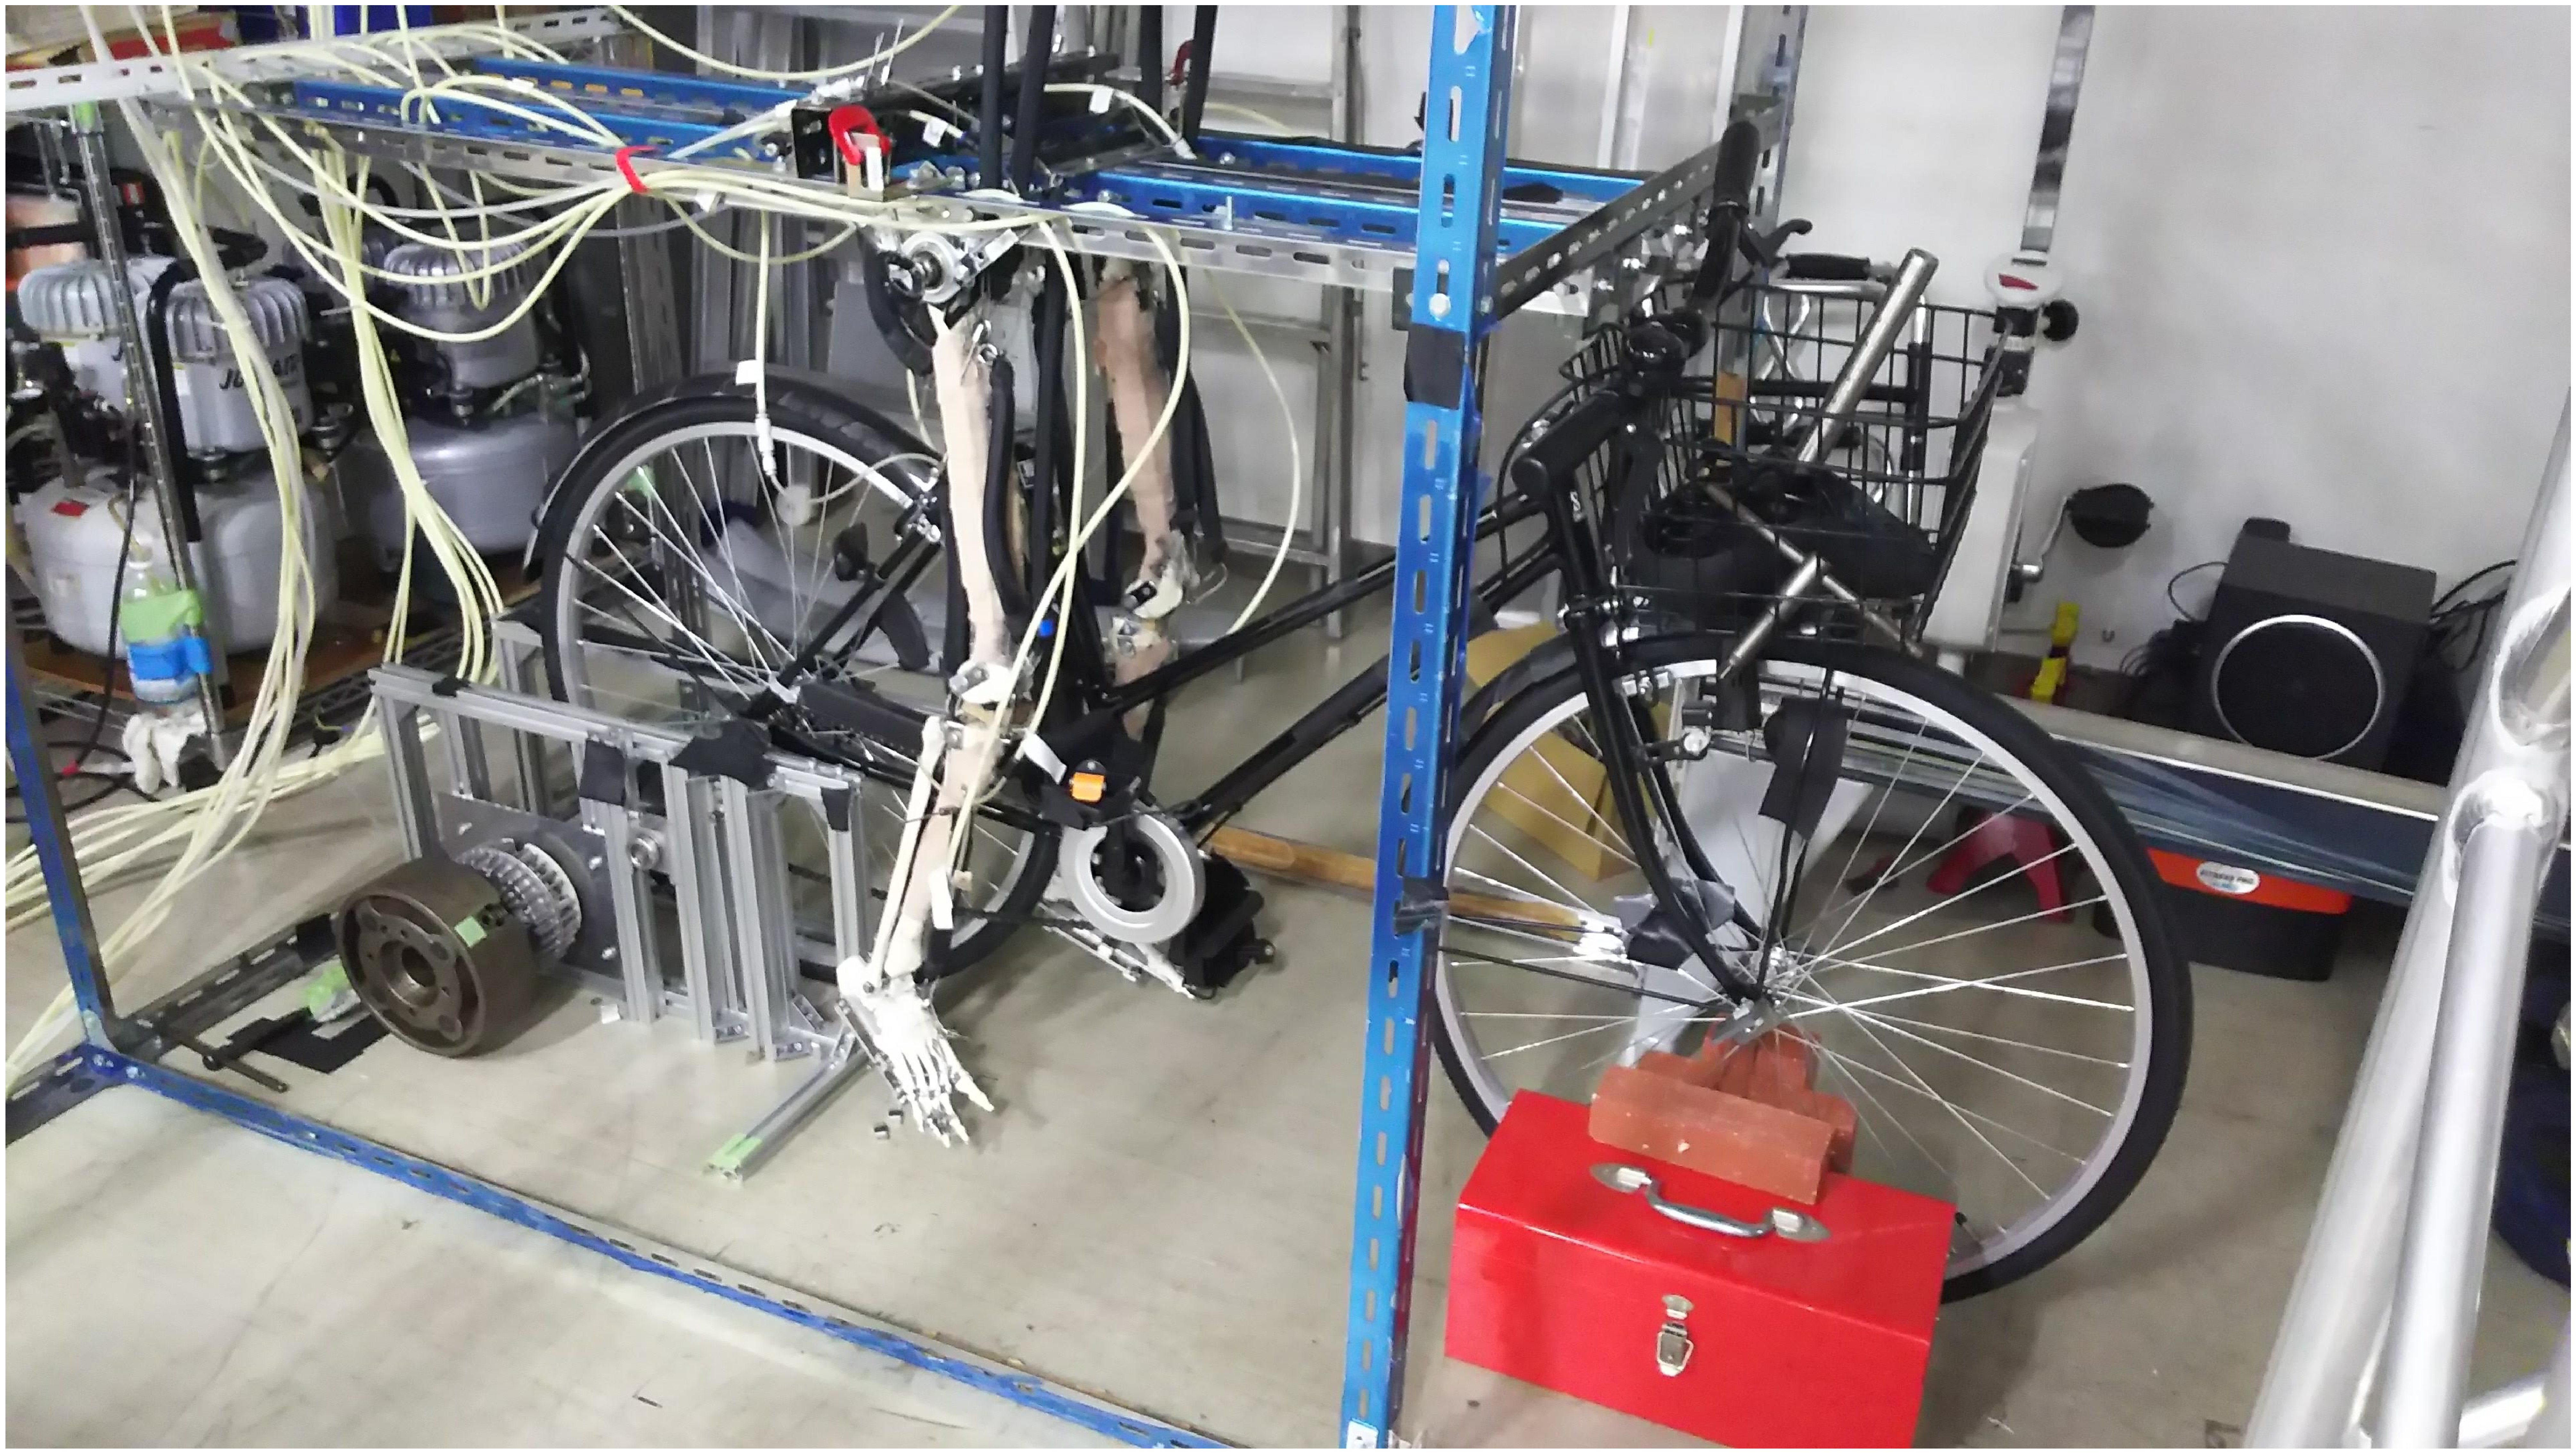
\includegraphics[width=0.75\columnwidth,clip]{1st.eps}
  \caption{ペダリングロボット(初号機)}
  \label{初号機}
  \end{center} %
\end{figure}

\newpage

\subsection{二足歩行ロボット}
%TODO:2号機のお話を書く
%TODO:2号機関連の研究のリファレンスを貼る
先述のペダリングロボットの研究成果を生かし、腰椎を固定していない状態の二足歩行ロボットが製作された。
本ロボットは、腰椎が固定されていないことにより立脚時の歩容動作の再現を行えるようになった。
なお、動作時は自重を支えることができないため、股間部の支持を行った。また、関節動作に関しては
先述のロボットと同様の形となっており,股関節,膝関節,足首関節それぞれがピッチ方向にのみ自由度を持っており
2次元平面上における動作を再現することが出来た.これらの動作の再現を行うため、空気圧人工筋が
ヒラメ筋,前脛骨筋,大腿四頭筋,大腿二頭筋,腸腰筋,恥骨筋の6筋分が搭載された形となっている.

これらの研究によって平衡点仮説に基づく筋シナジー解析を用いた歩行動作の解明の為に用いられた。
この歩行動作解析により、健常者の歩行と片麻痺患者の歩行の動作の相違に関して解明することができた。
\begin{figure}[h]
  \begin{center}
  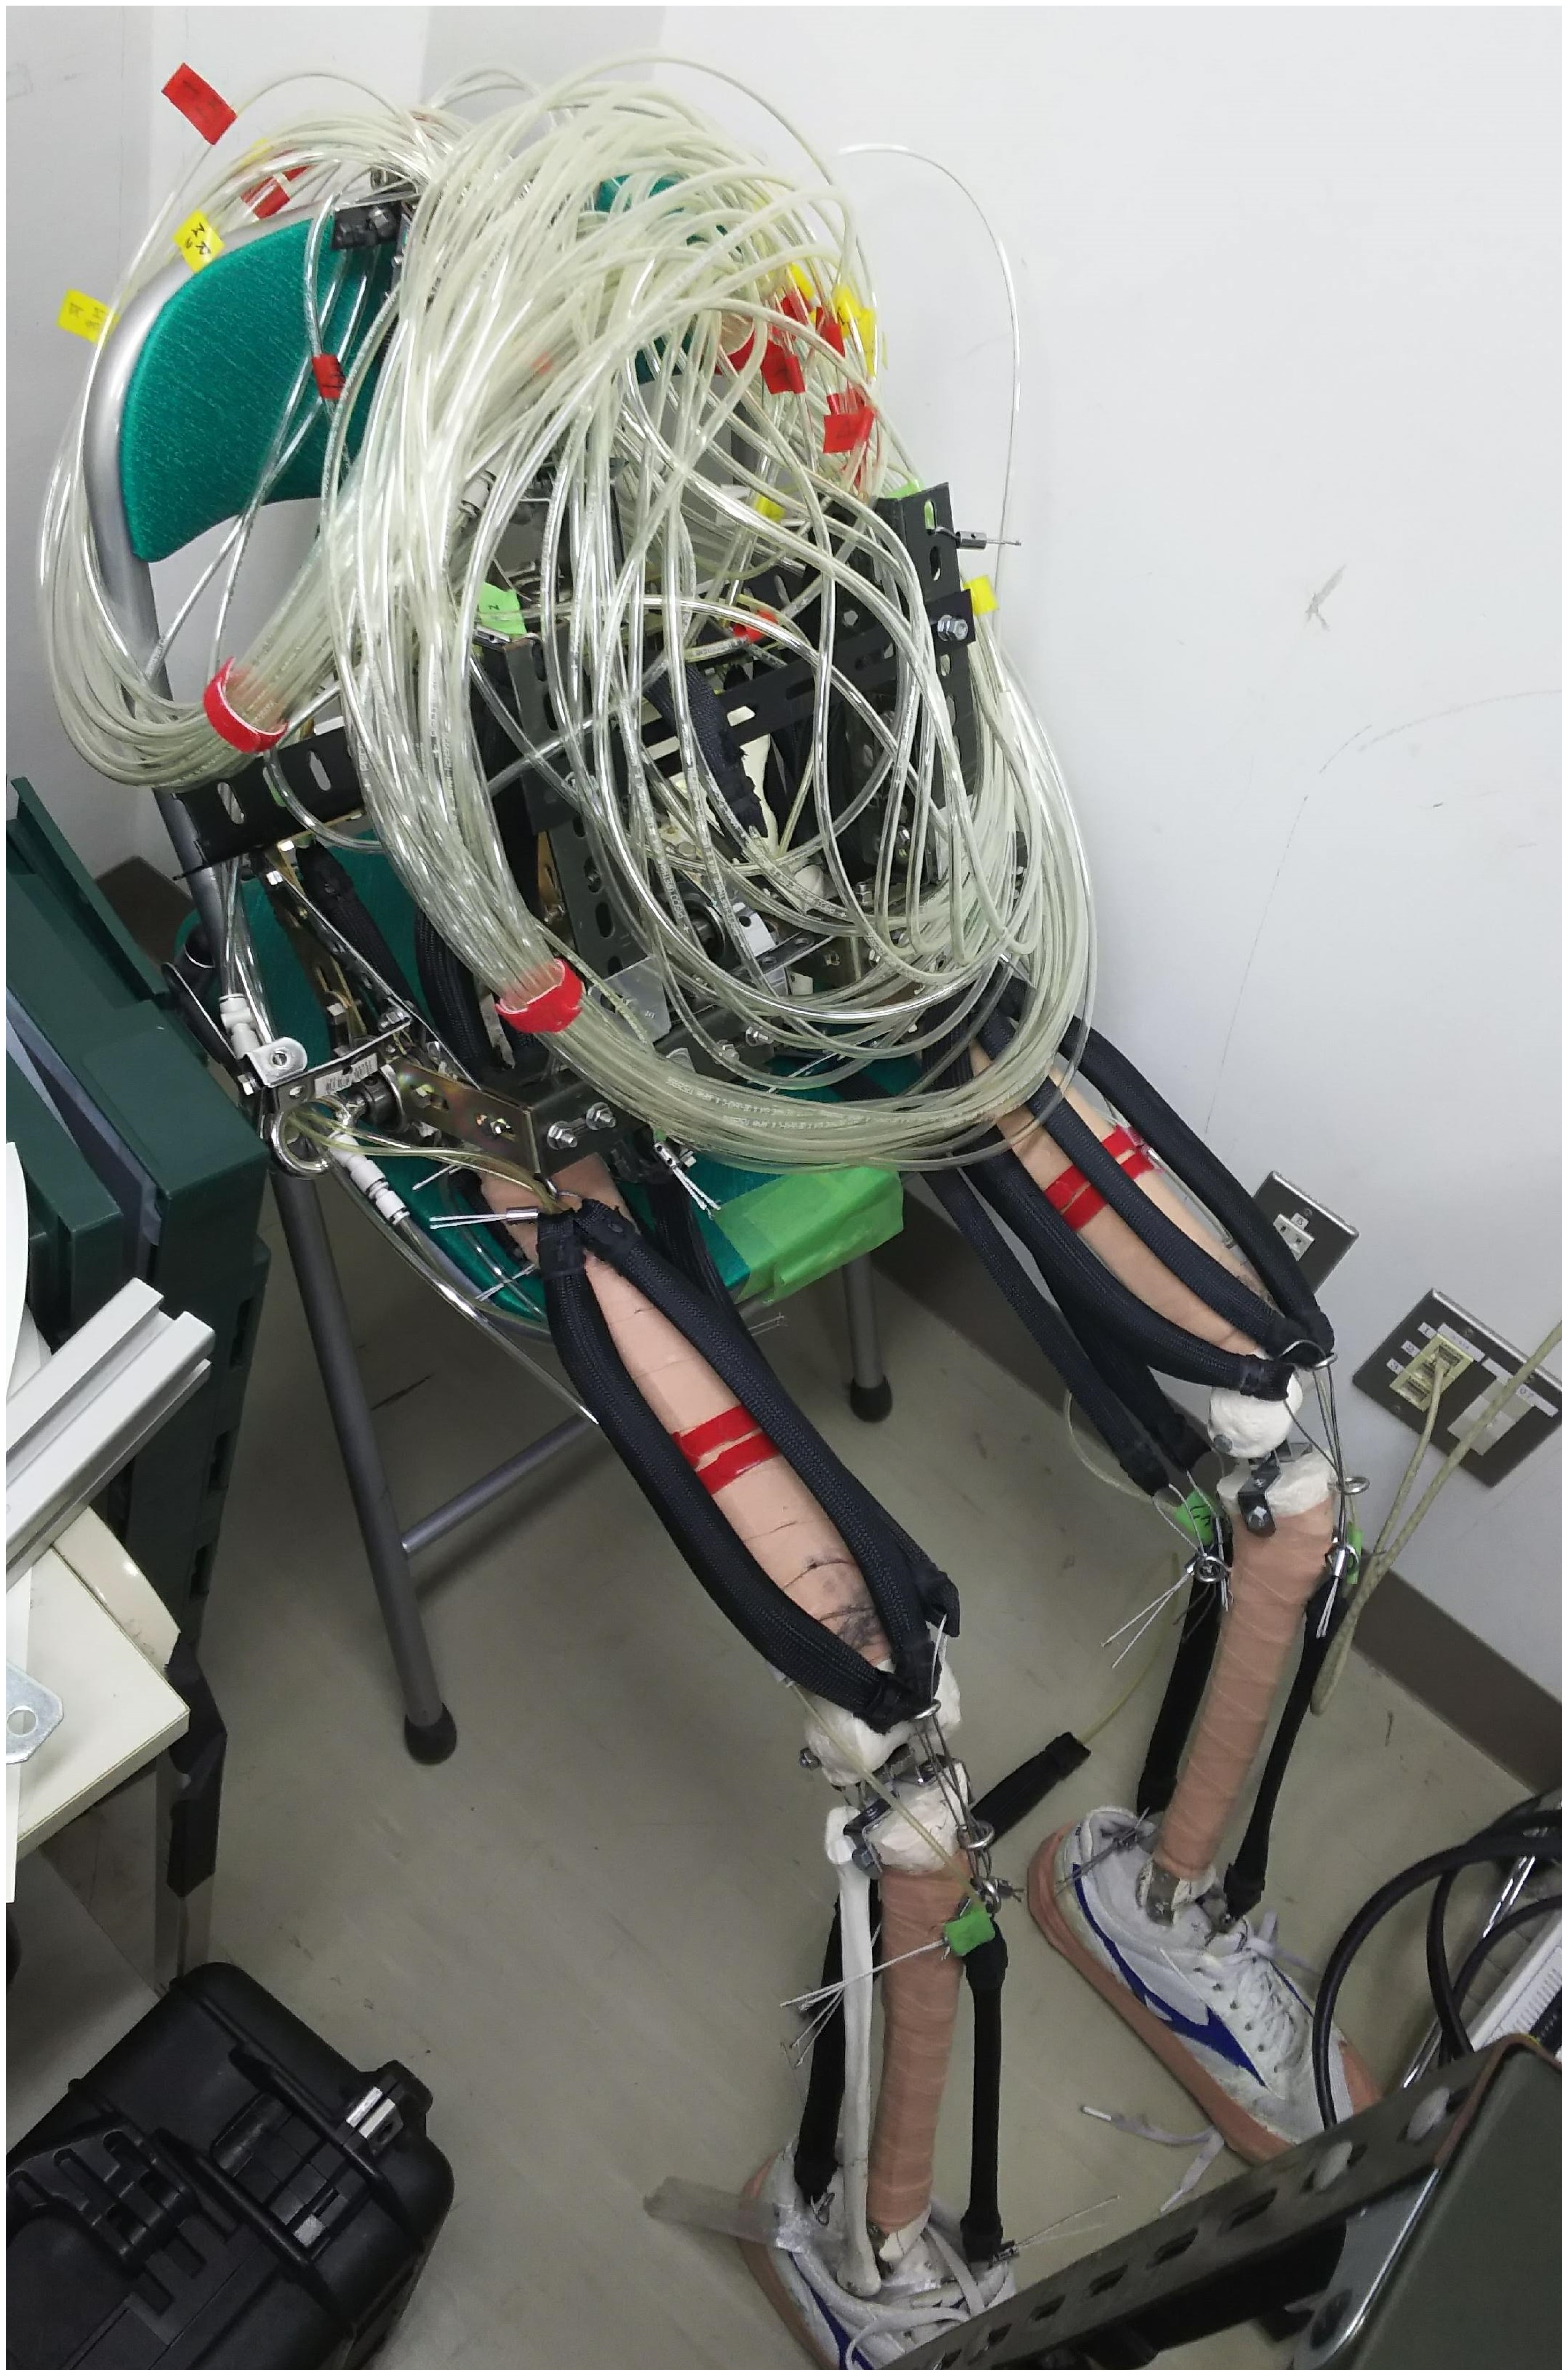
\includegraphics[width=0.35\columnwidth,clip]{2nd.eps}
  \caption{二足歩行ロボット(2号機)}
  \label{2号機}
 \end{center}
\end{figure}

\newpage

\subsection{柔軟性の高い伸縮センサ}%TODO:伸縮センサのお話を書く
soft robotics toolkit\cite{MITSoftRobot}において,シリコンと導電性布をもちいた伸縮センサが
紹介されている.本センサは,伸縮性に優れており,柔軟性も兼ね備えたものとなっている.また,
製作コストも\$23と非常に安価なものであると紹介されている.

今回は,このセンサーとその計測系を作成し,空気圧人工筋を用いた足関節ロボットに搭載し,
空気圧人工筋の伸展の計測を行うことを目標とする.
\begin{figure}[h]
    \begin{center}
        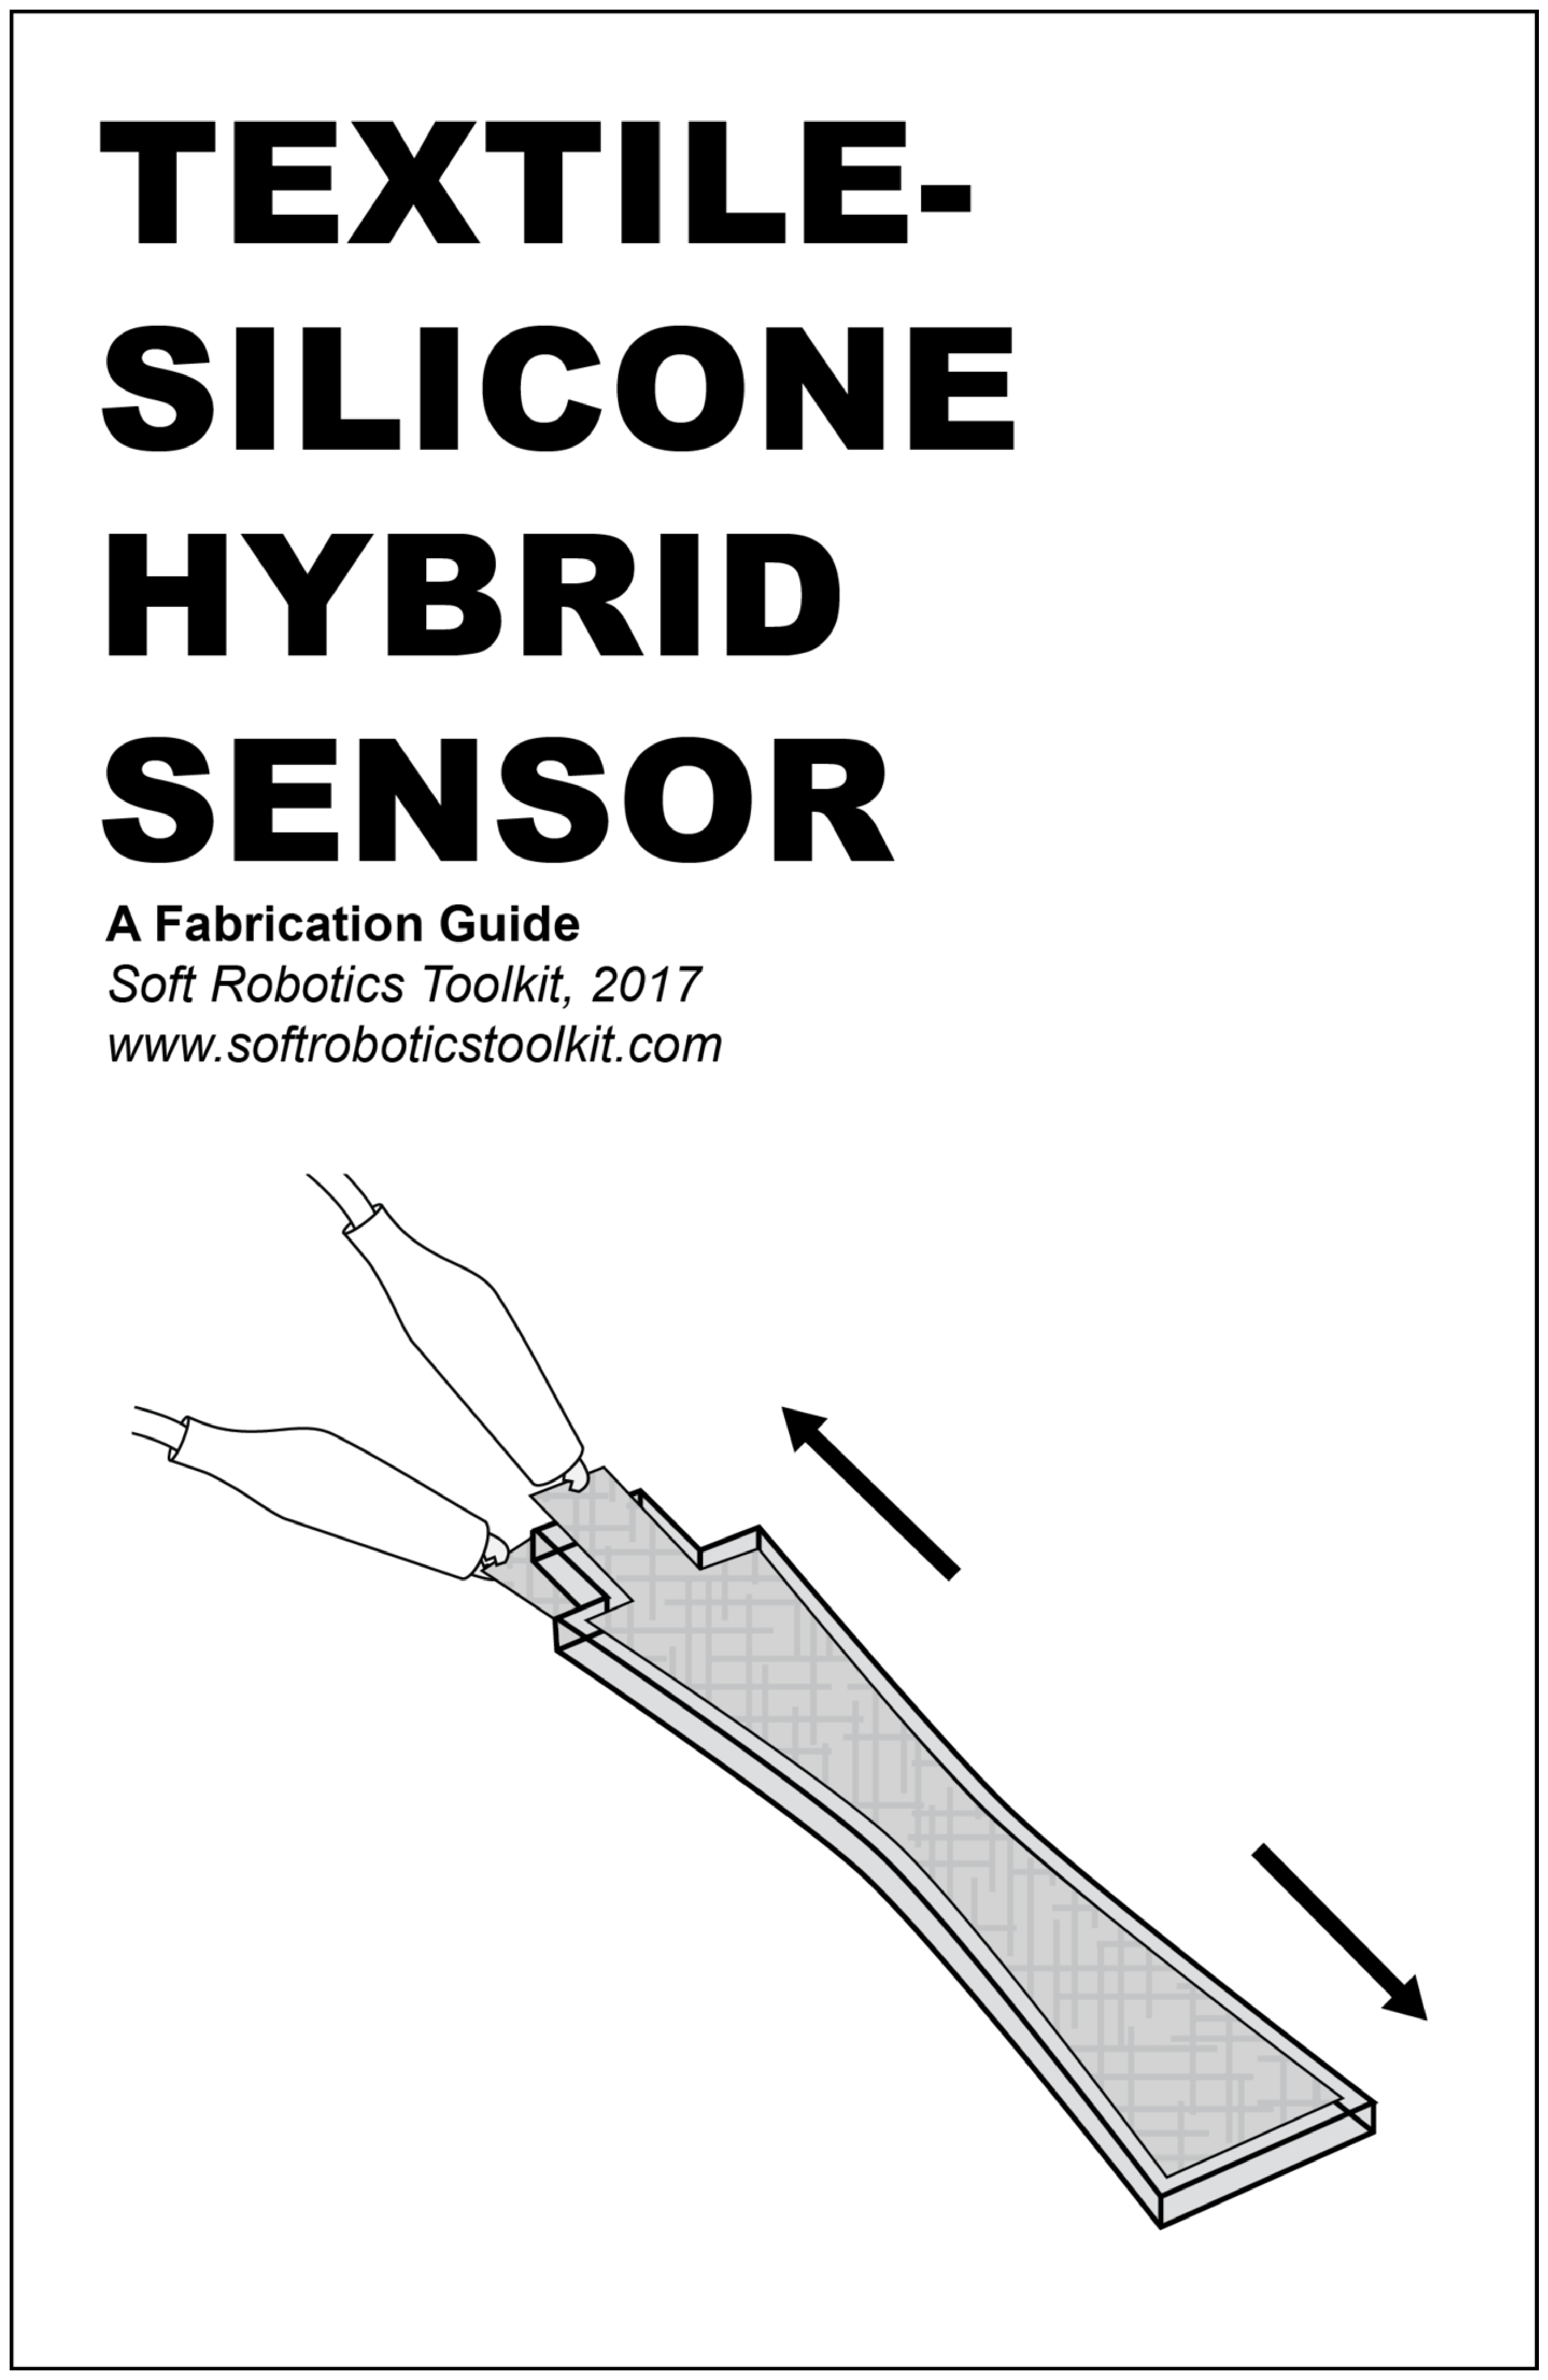
\includegraphics[width=0.5\columnwidth]{./MITSoftRobotics.eps}
        \caption{伸縮センサ模式図\cite{MITSoftRobot}}
        \label{MITSoftRobot表紙}
    \end{center}
\end{figure}

%TODO:3号機のお話を書く

\section{研究目的}
%TODO:これらを統合し,筋肉の伸長を巻き込んだシステムの話をする

先述の,ペダリングロボット(初号機),2足歩行ロボット(2号機)の経験を踏まえ,今回新たに2足歩行ロボット(3号機)の開発を行った.従来の2足歩行ロボットでは自由度の制約が大きく,2次元平面上のみでの動作となっていたものが3次元空間上で動かせるものとした.

股関節部分の自由度

足関節の自由度が従来の2足歩行ロボット(2号機)ではピッチ方向の1自由度であった.一方で実際の人間の自由度はこれに加えてロール方向,ヨー方向も存在し3自由度である.

今回開発を行った導電性布,シリコンを用いた伸縮センサを空気圧人工筋に組み合わせ


\section{論文構成}
本論文の構成は以下の通りである.
{\bf 第2章}で足関節ロボット、伸縮センサの製作過程と伸縮センサにおけるデータ処理について述べ,{\bf 第3章}でその解析結果を示す.
{\bf 第4章}では考察する. %TODO考察内容の記述を行う
最後に{\bf 第5章}で本論文の成果をまとめる.

\chapter{実験方法}
\section{動作モデル}
\subsection{足首}
%TODO:足首周りの動作関係のお話をする
%付着筋肉のお話もする
付着筋肉 %何の筋肉をもちいた?

ボールジョイントを用いて,ロール・ピッチ・ヨー各軸に自由度を持たせた.

\subsection{伸縮センサ}
%TODO: 大学PCで書いた伸縮センサCADのレンダリング画像を挿入する
伸縮センサはFig.\ref{伸縮センサ断面図}において示す通り,柔軟で弾性変形する伸縮性シリコン(絶縁層)と導電性布電極(導電層)の重ね合わせによって構成されている.これは,誘電体をシリコン,極板を導電性布としたコンデンサとなっている.

\begin{figure}[h]
    \begin{center}
        \label{伸縮センサ全体図}
        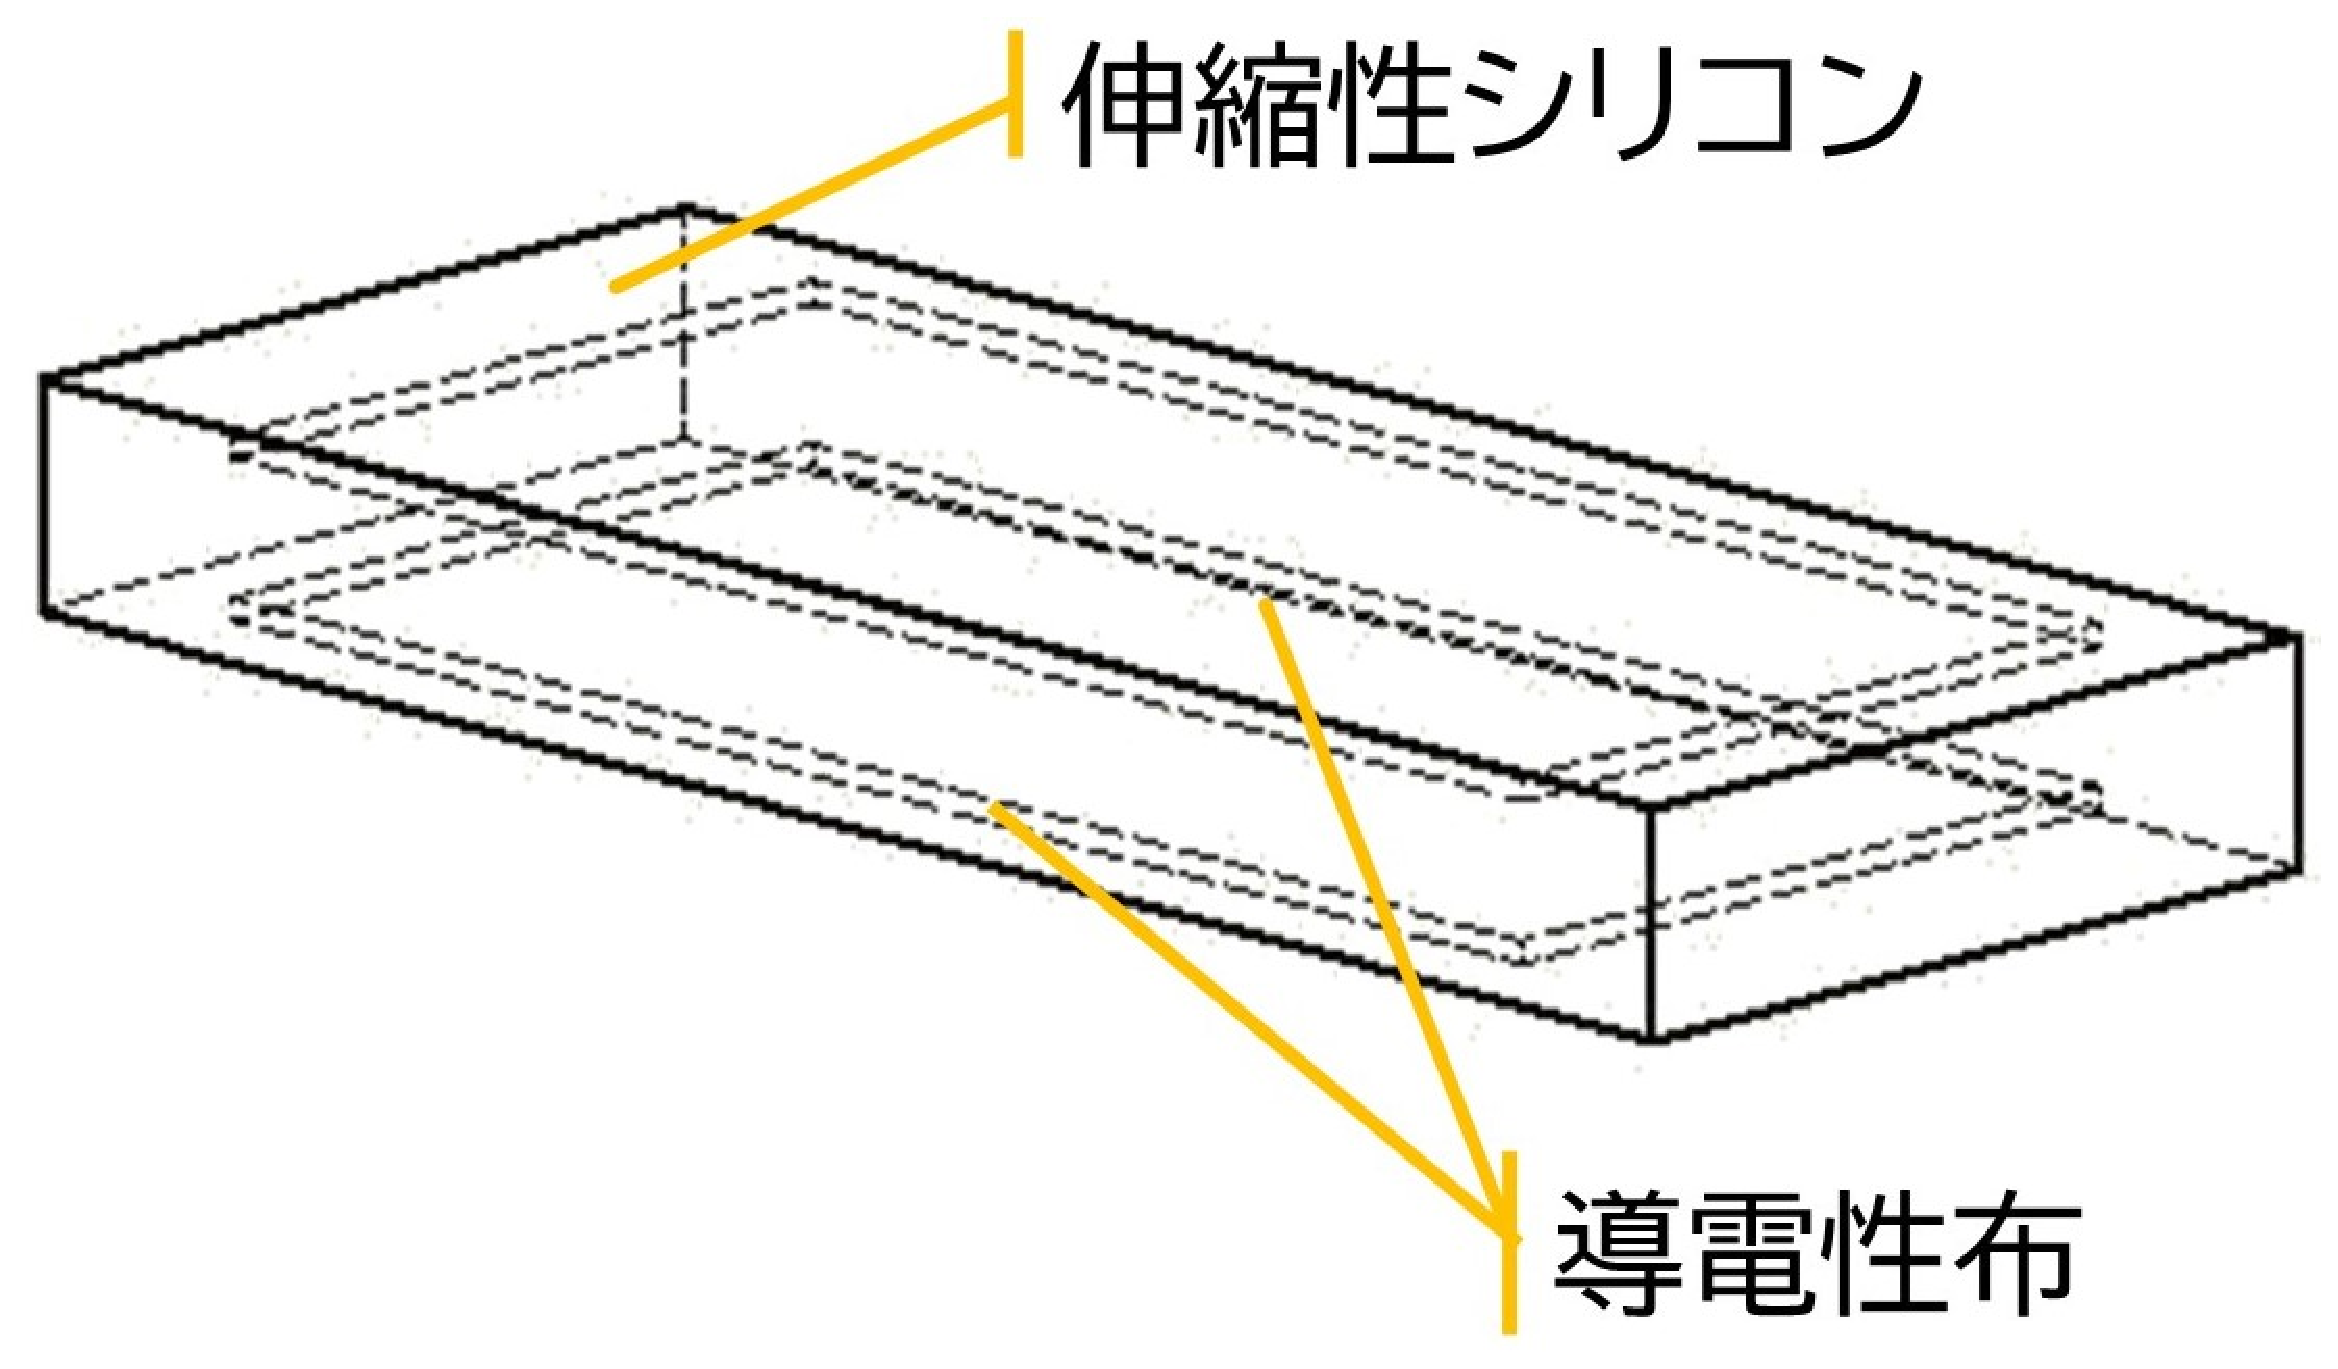
\includegraphics[width=0.85\columnwidth,clip]{Photo/BackGround/画像_説明付き/スライド1.eps}
        \caption{伸縮センサ全体図}
    \end{center}
\end{figure}
\begin{figure}[h]
    \begin{center}       
        \label{伸縮センサ断面図}
        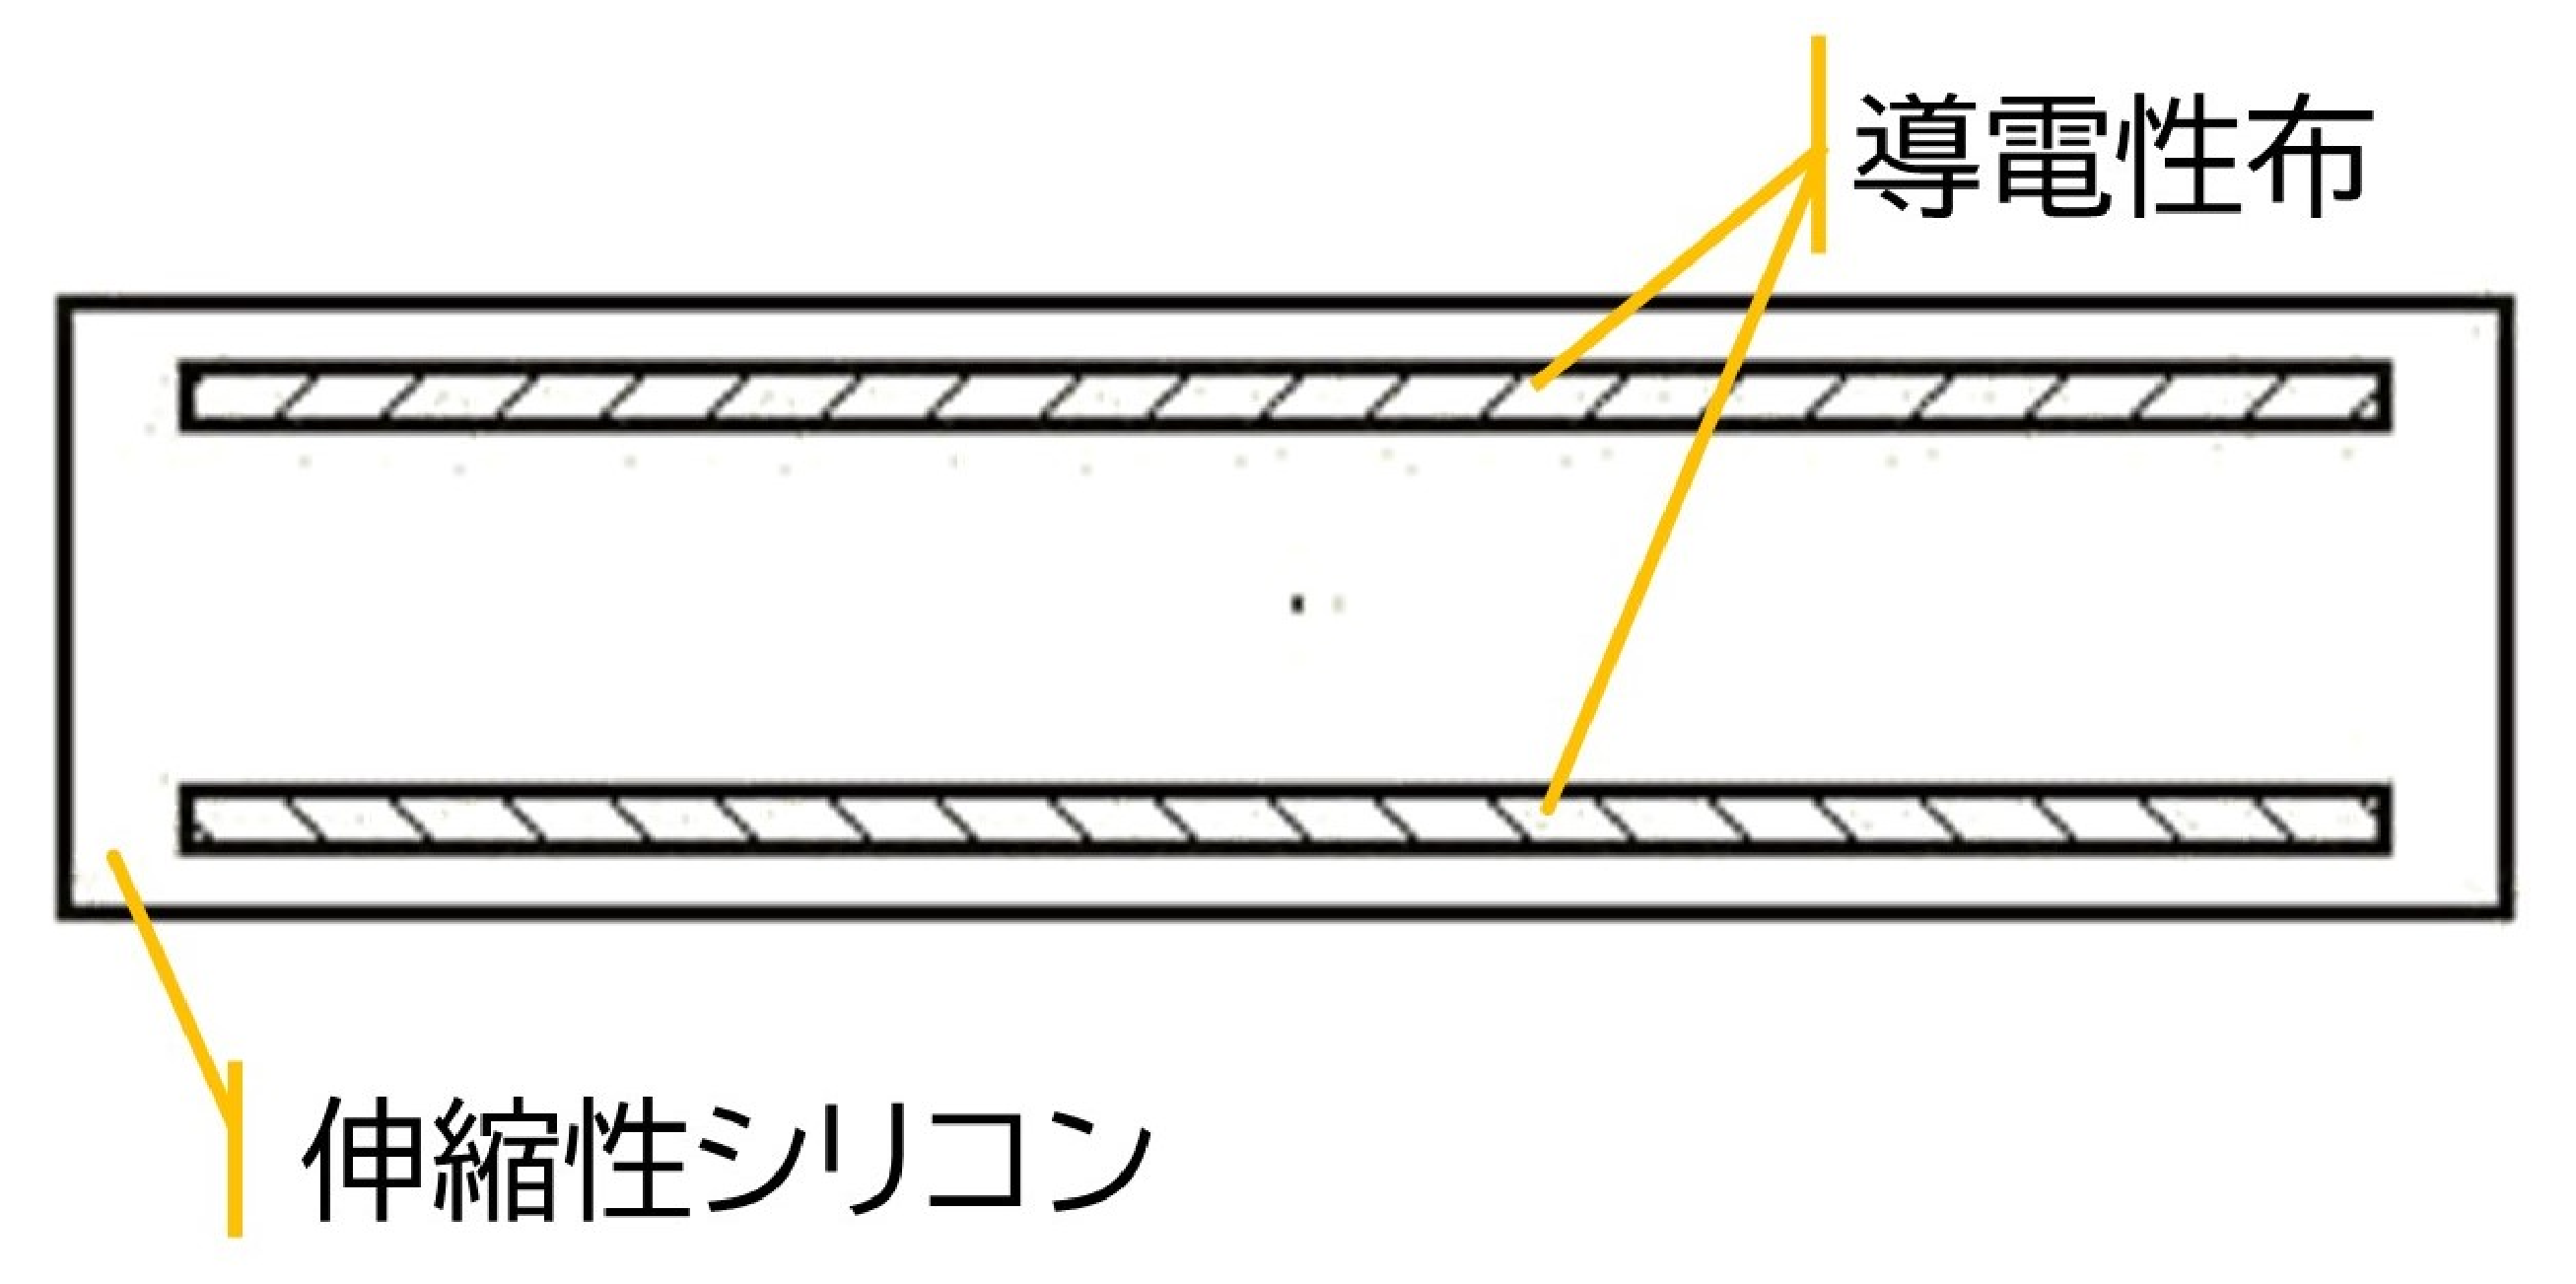
\includegraphics[width=0.85\columnwidth,clip]{Photo/BackGround/画像_説明付き/スライド2.eps}
        \caption{伸縮センサ断面図}
    \end{center}
\end{figure}

ここで伸縮センサ中の導電性布の表面積$S$,誘電体の厚さを$d$,真空の誘電率を$\epsilon{}_0$,シリコンの比誘電率を$\epsilon{}_s$とすると,
\begin{eqnarray}
    C=\epsilon{}_0\epsilon{}_s\frac{S}{d}
\end{eqnarray}
といった式となる.ここで体積が一定の変化であると仮定すると, 

ここで静電容量の変化を$\Delta{}C$,厚みの変化を$\Delta{}d$とそれぞれすると、

一方で,伸縮センサは引張方向のみに応力がかかる単軸応力状態であると見れるため,引張方向のひずみ$\gamma$,引張方向の垂直応力$\sigma$,ヤング率$E$とそれぞれすると,
\begin{eqnarray}
    \sigma=E\gamma
    \label{フックの法則}
\end{eqnarray}
といった式がフックの法則により示される.また,引張方向に対して直交方向である垂直ひずみ$\gamma{}_s$,ポアソン比$\mu$とすると,
\begin{eqnarray}
    \mu = \frac{\gamma{}_s}{\gamma}
    \label{ポアソン比}
\end{eqnarray}
といった式となる.

\subsection{伸縮センサ計測回路}
%TODO:伸縮センサ計測回路に関しての記述を行う
%TODO:RC回路の電圧を掛けたときの時定数の様子をオシロスコープで撮影した画像が欲しい
伸縮センサは静電容量の変化で伸縮状況を示す.故に今回は静電容量の変化を計測することができるシステムを用いればよい.そのため,NucleoF303K8にRC回路を用いて可変静電容量に関して,固定抵抗器を用いて計測を行った.

\begin{figure}[h]
 \begin{center}
    %Voutの向きを出力にする
  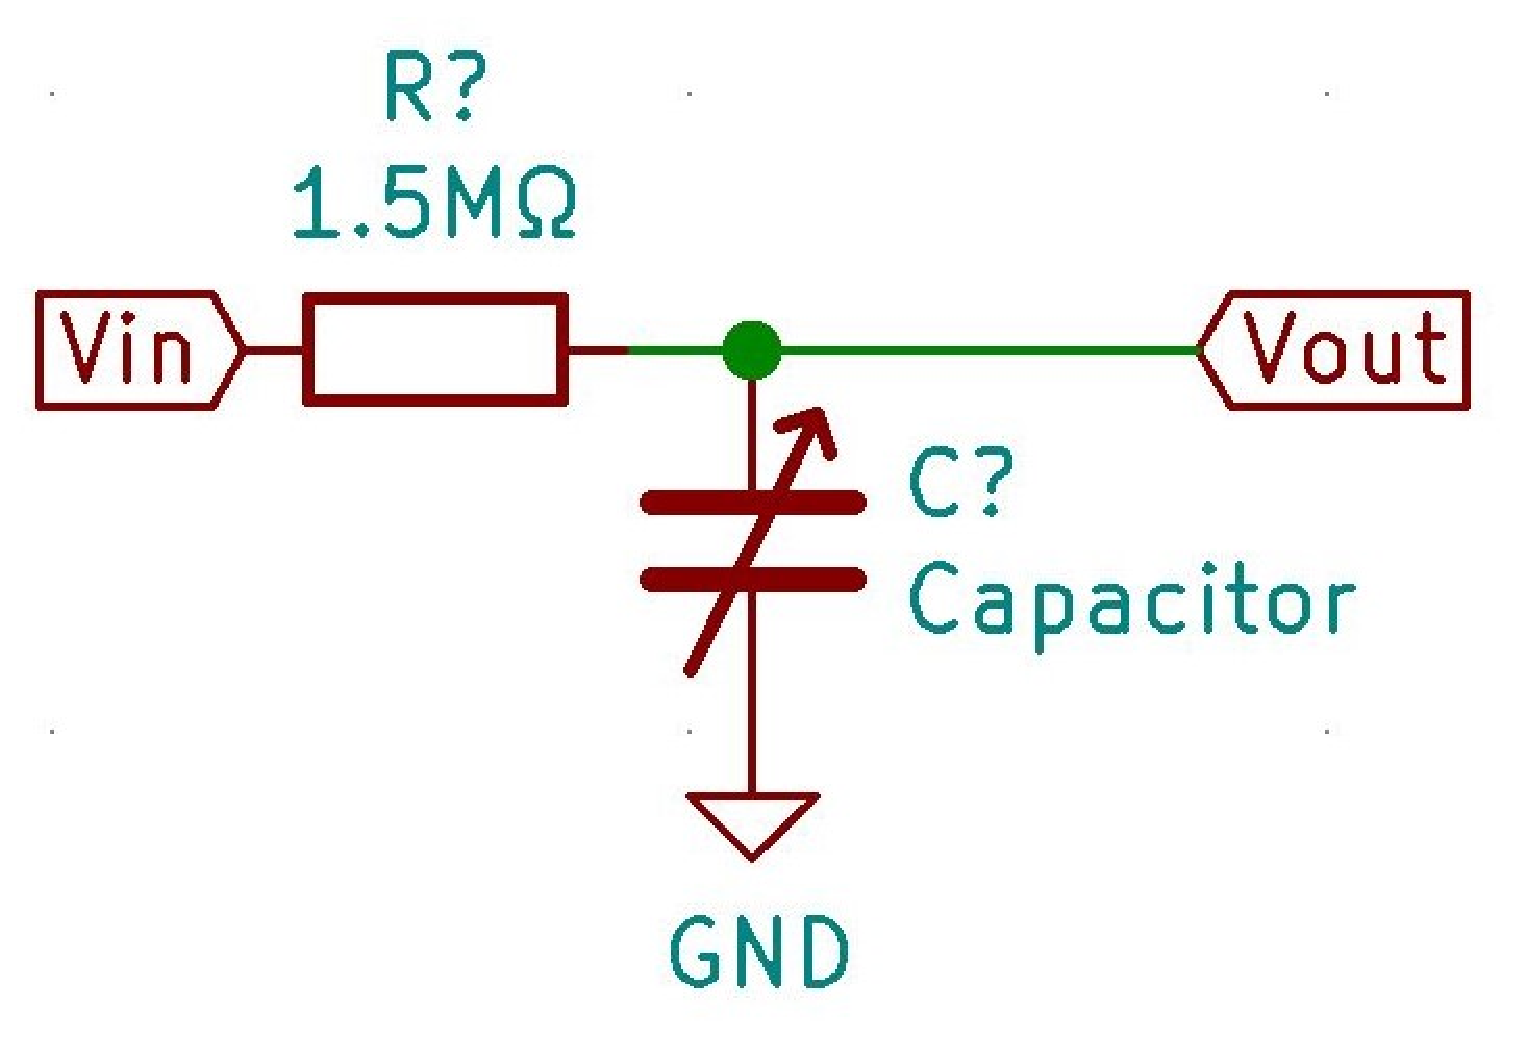
\includegraphics[width=0.75\columnwidth,clip]{Photo/BackGround/RC.eps}
  \caption{RC回路}
  \label{RC}
 \end{center}
\end{figure}

これらの計測に関して,1つのマイコンを用いて複数の伸縮センサの計測を行うと計測周期が低下し,計測精度の低下が懸念された.これを踏まえ,1つのマイコンで計測を行う伸縮センサの数を2個とした.一方で今回,足首を中心とした筋の伸縮の計測を行うため6チャンネル分の計測を行う必要がある.故に,マイコン3枚分の計測システムを用意した.これらをCAN通信(Controller Area Network)と同期信号を用いて計測のデータ取得,同期を行った.
\begin{figure}[h]
 \begin{center}
  
\includegraphics[width=0.75\columnwidth,clip]{Photo/BackGround/circuit.eps}
  \caption{計測時に実際にもちいた基板}
  \label{circuit}
 \end{center}
\end{figure}
\chapter{解析方法}
\section{ストレッチセンサ計測アルゴリズム}
\ref{sec:RC回路}にて示す通り、ストレッチセンサの静電容量変化の計測にはRC回路を用いた時定数の計測で行った。
なお、この時定数の計測にはNucleoF303K8といったマイコン評価ボードを使用した。また、それらのコードの記述にはmbedライブラリを使用した。
使用したソースコードは下記リンクにて公開している。計測アルゴリズムはFig.\ref{fig:algorithm}にて示すように
1000Hzで計測を実行し、100Hzごとに計測データの平均値をSerial通信を用いてPCに出力した。
また、2000Hzで出力ピンの状態を切り替え、ストレッチセンサに電荷が残らないようにした。

ソースコード:https://os.mbed.com/users/HidetoN/code/Cap-Sensor/

\begin{figure}[h]
    \begin{center}
     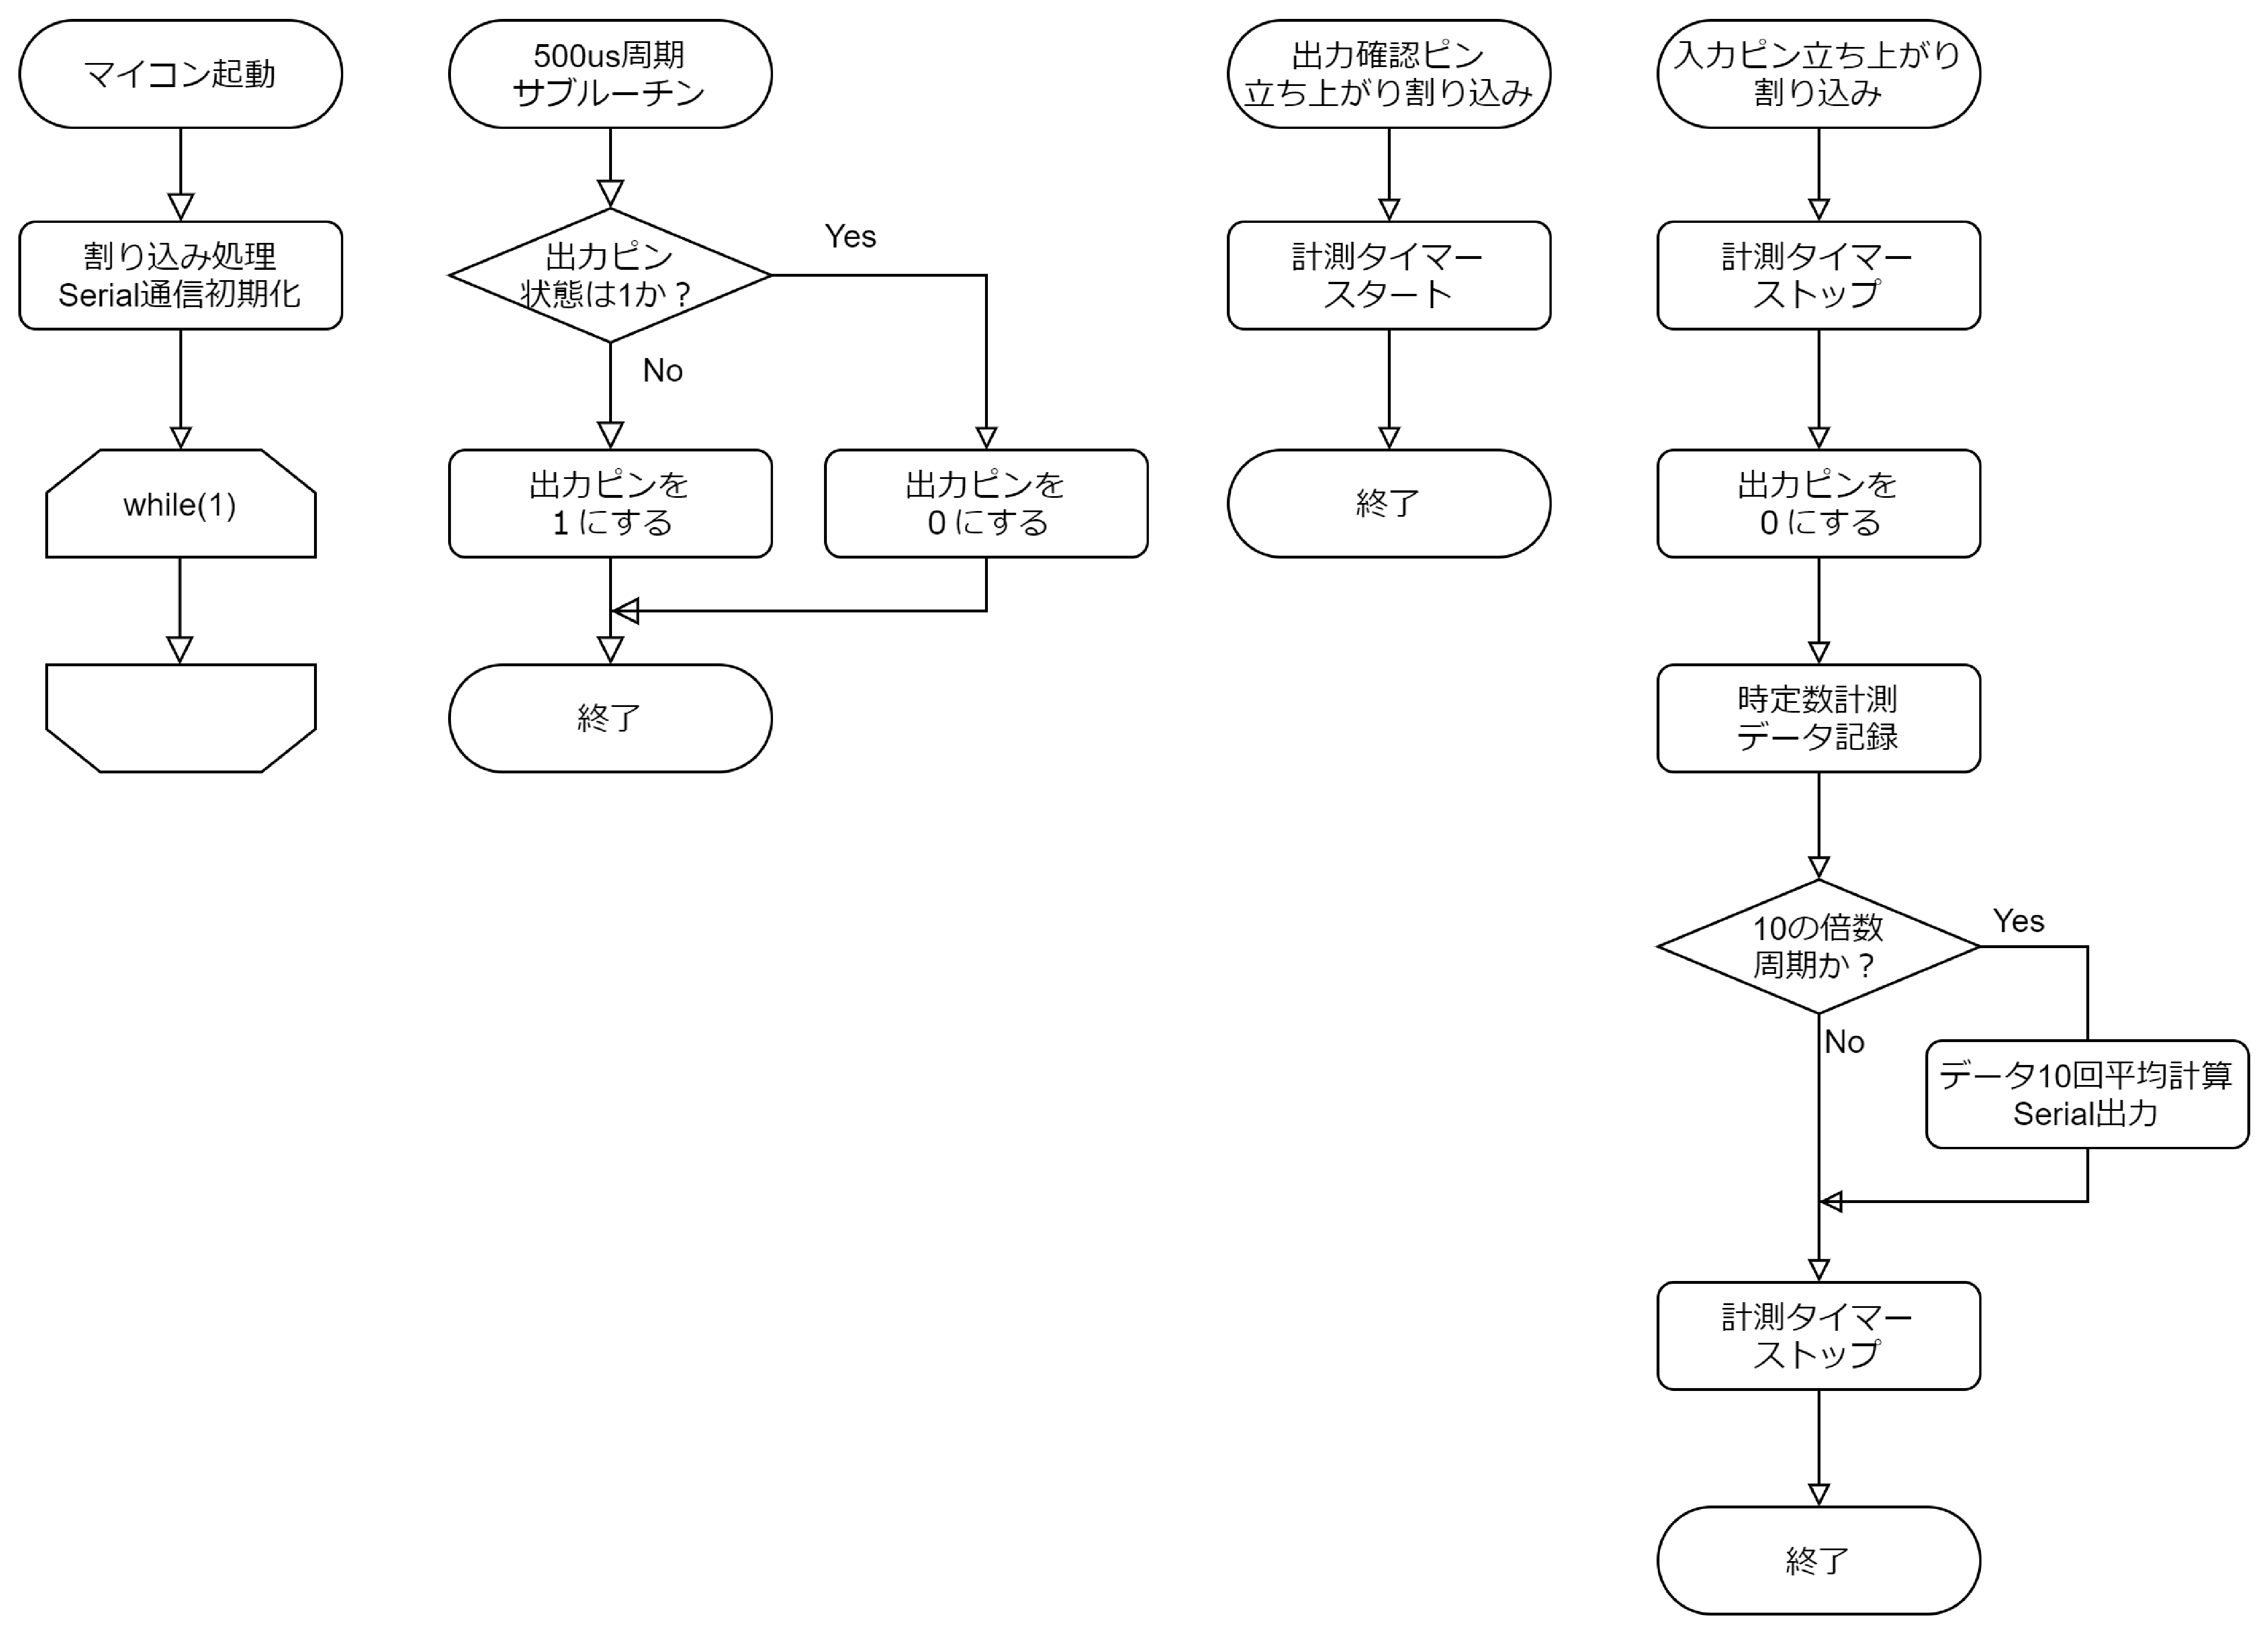
\includegraphics[width=0.9\columnwidth,clip]{./3_analysis/algorithm.eps}
     \caption{計測プログラムにおけるアルゴリズム}
     \label{fig:algorithm}
    \end{center}
\end{figure}

\section{足関節ロボット駆動システム}
足関節ロボットの駆動システムには従来から存在するペダリングロボット、2足歩行ロボットのシステムと同様のシステムを利用した。
以下にそのシステムに関して記述する。

%TODO:システムブロック図入れられると入れたい...
まず、Fig.\ref{fig:compressor}にて示す、エアーコンプレッサーで8気圧まで圧縮空気を作成し、気圧調整弁を用いて6気圧まで減圧を行った。
続いて、制御用PCに搭載されたDAボードより、空気圧制御盤にアナログ信号を送信する。なお、この電圧指令は550段階で制御が行うことが出来る。
この電圧指令を元に空気圧制御盤に搭載された空気圧制御器によって可変的に空気圧の制御を各人工筋に対して行う。

\begin{figure}[h]
    \begin{center}
     
\includegraphics[width=0.65\columnwidth,clip]{./3_analysis/compressor.eps}
     \caption{使用したエアーコンプレッサー}
     \label{fig:compressor}
    \end{center}
\end{figure}

\begin{figure}[h]
    \begin{center}
     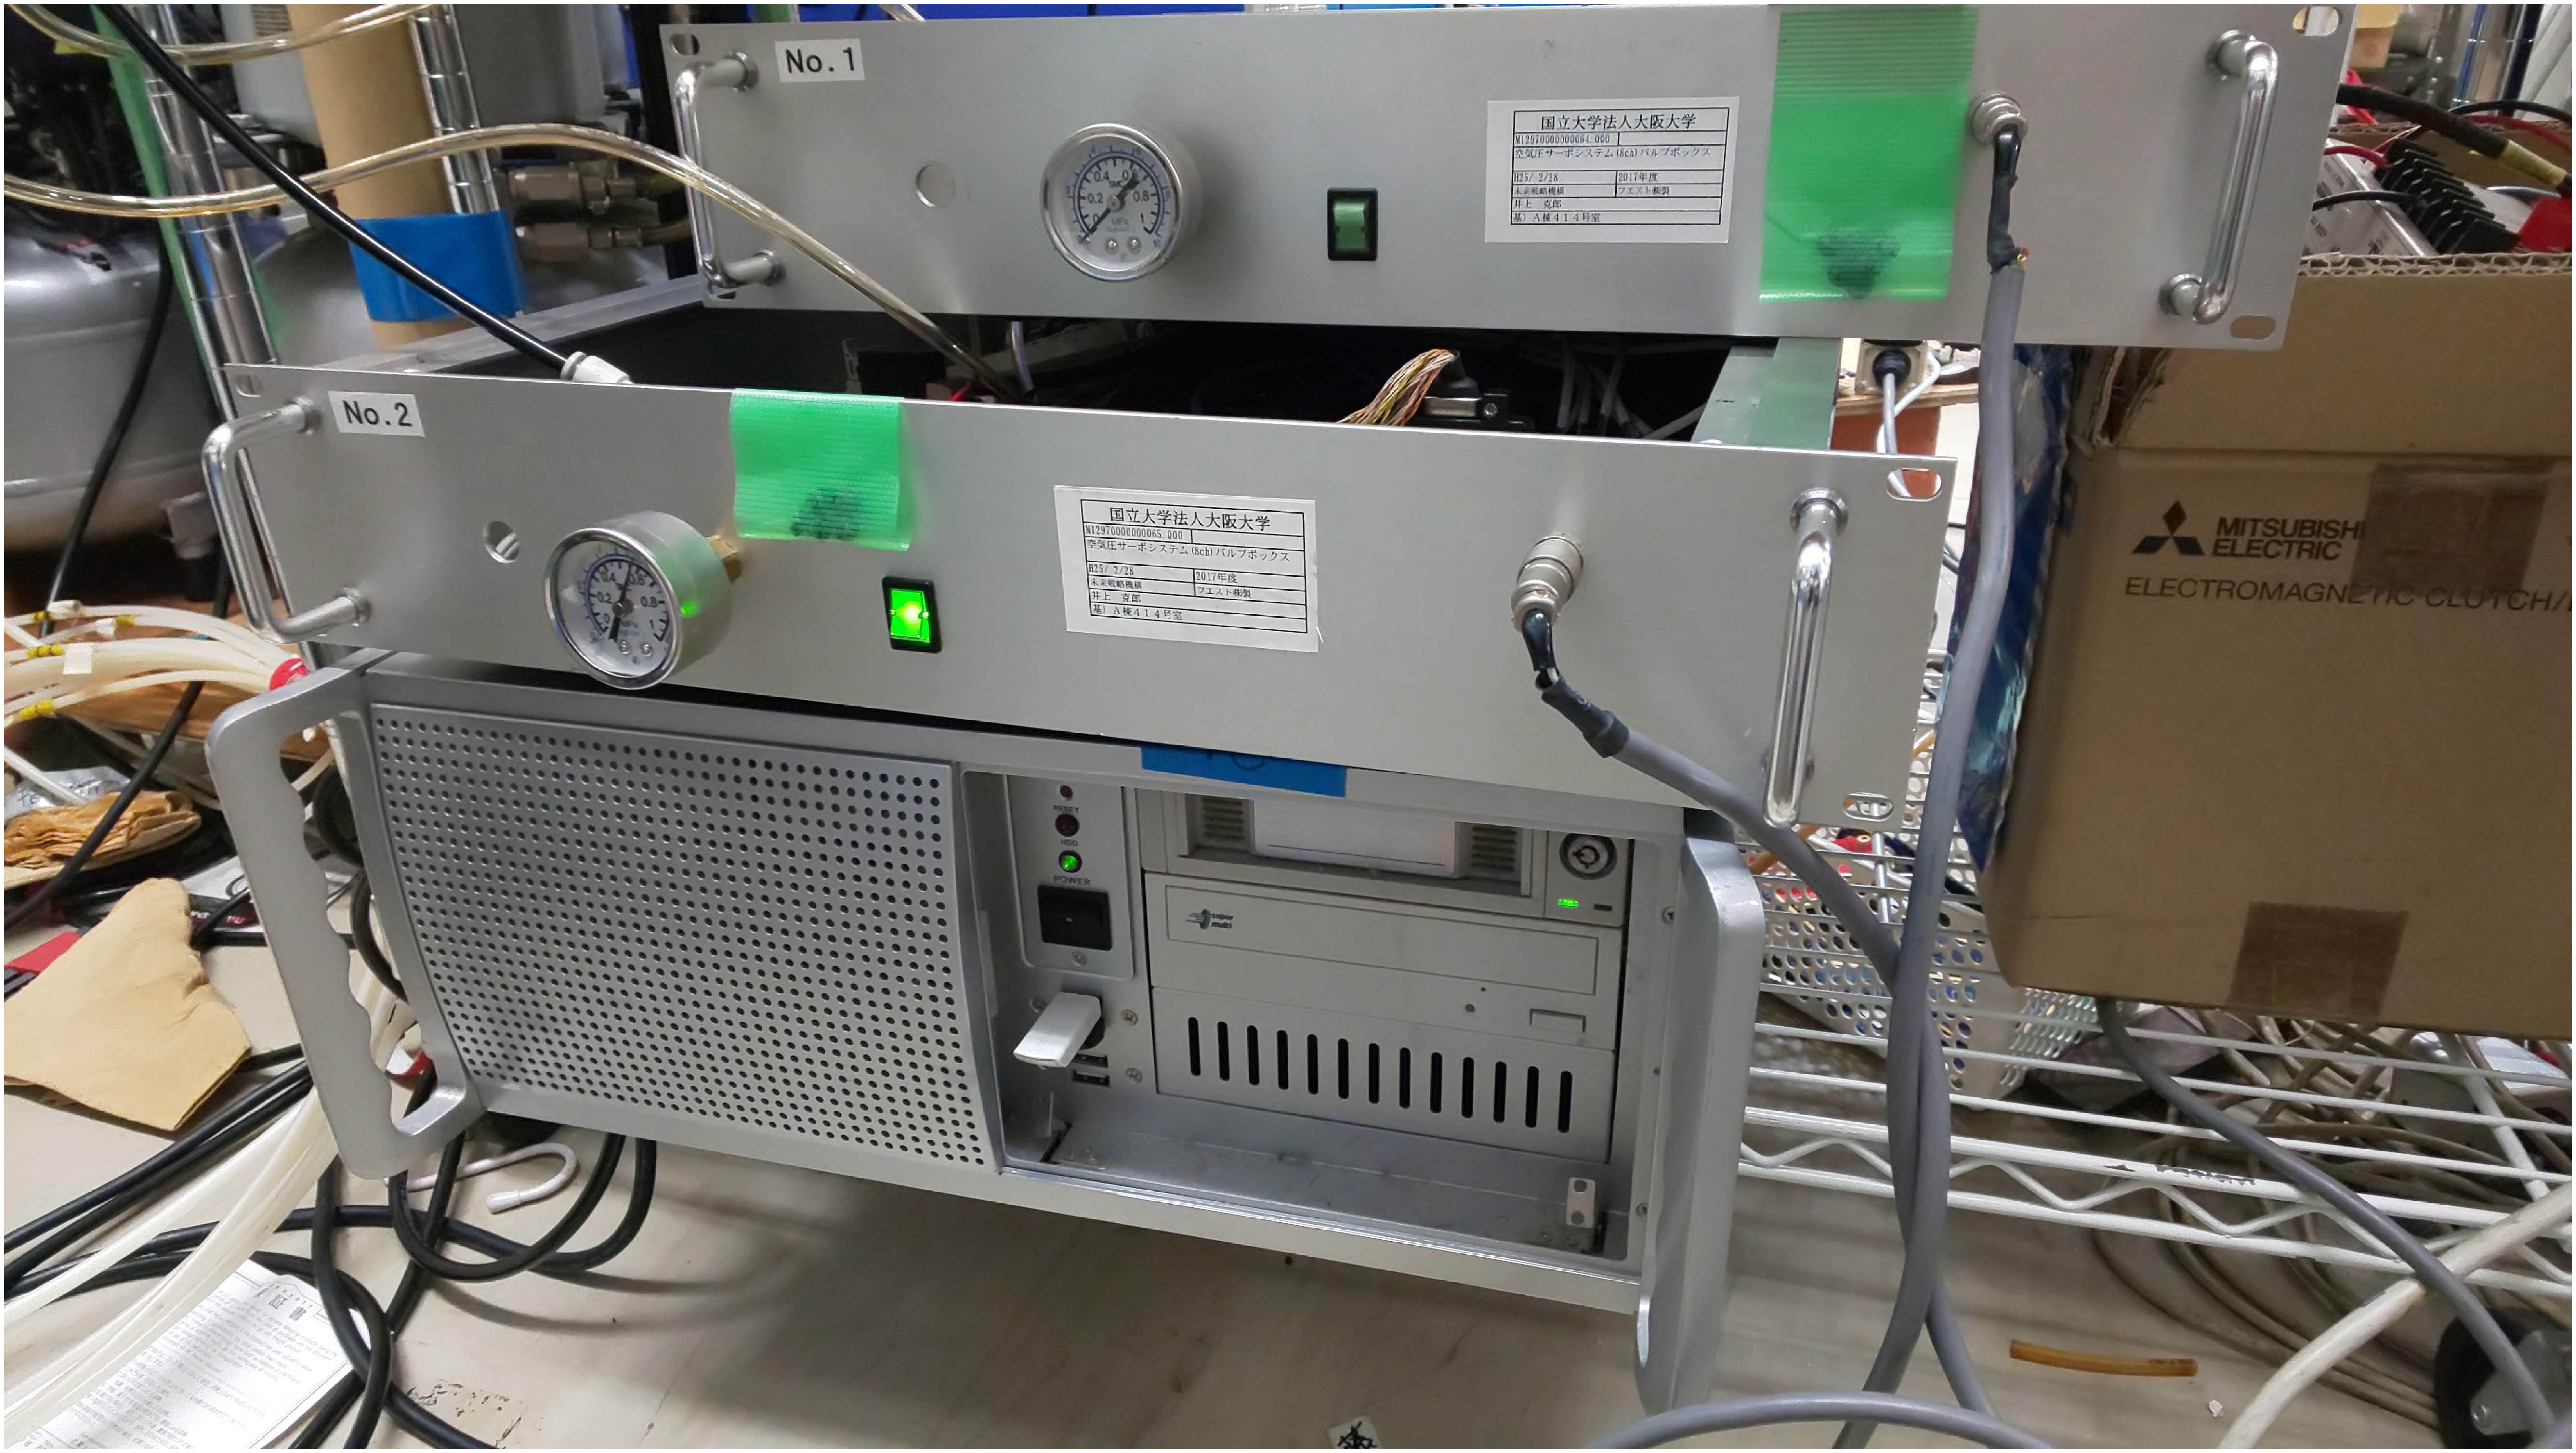
\includegraphics[width=0.65\columnwidth,clip]{./3_analysis/PC.eps}
     \caption{制御PCとエアー制御盤}
     \label{fig:PC}
    \end{center}
\end{figure}

\section{ストレッチセンサ計測データ処理}
ストレッチセンサの計測データはNucleoF303K8よりSerial通信によって921600bpsで出力される。
制御アルゴリズムの部分でも示したが、1000Hz周期で取得したデータの平均値が100Hz周期に出力される。
このデータをTeraTermのログ取得機能を用いてcsvファイルとして保存した。
なお、足関節ロボット制御用PCの処理の都合上、別PCを用いて結果の取得を行った。

\chapter{結果・考察}
\section{結果}
\subsection{ストレッチセンサ計測精度評価}
Fig. \ref{output_for_test}のような出力を各空気圧人工筋に与えた結果,
Table.\ref{strain}のような長さの結果となった.
また,それぞれの時におけるストレッチセンサ時定数の結果を求めると,Table.\ref{4_2}に示す様になった.
\begin{table}[h]
    \caption{ストレッチセンサ 長さ(mm) 計測結果}
    \label{strain}
    \begin{center}
        \begin{tabular}{|c|c|ccc|}\hline
            \multicolumn{2}{|c|}{} & \multicolumn{3}{c|}{筋肉種類}\\
            \cline{3-5}
            \multicolumn{2}{|c|}{} & 前脛骨筋 & 腓骨筋 & ヒラメ筋 \\ \hline
            & 1 & 236 & 194 & 208 \\ \cline{2-5}
            & 2 & 234 & 197 & 210 \\ \cline{2-5}
            & 3 & 233 & 198 & 213 \\ \cline{2-5}
            & 4 & 234 & 199 & 214 \\ \cline{2-5}
            & 5 & 220 & 204 & 215 \\ \cline{2-5}
            計測位置 & 6 & 208 & 217 & 225 \\ \cline{2-5}
            & 7 & 214 & 217 & 227 \\ \cline{2-5}
            & 8 & 215 & 215 & 223 \\ \cline{2-5}
            & 9 & 218 & 203 & 218 \\ \cline{2-5}
            & 10 & 233 & 195 & 216 \\ \cline{2-5}
            & 11 & 234 & 192 & 212 \\ \cline{2-5}
            & 12 & 235 & 197 & 209 \\ \hline
        \end{tabular}
    \end{center}
\end{table}

\newpage

%セルを結合して中央揃え
%(参考):https://qiita.com/ta_b0_/items/c8c828b6a53d49498736
\begin{table}[h]
    \caption{ストレッチセンサ 時定数(us) 計測結果}
    \label{4_2}
        \begin{center}
            \begin{tabular}{|c|c|ccc|}\hline
            \multicolumn{2}{|c|}{} & \multicolumn{3}{c|}{筋肉種類}\\
            \cline{3-5}
            \multicolumn{2}{|c|}{} & 前脛骨筋 & 腓骨筋 & ヒラメ筋 \\ \hline
            & 1 & 43.86±0.02 & 68.14±0.03 & 40.13±0.01 \\ \cline{2-5}
            & 2 & 44.42±0.02 & 68.07±0.02 & 40.13±0.01 \\ \cline{2-5}
            & 3 & 44.73±0.02 & 68.07±0.02 & 39.26±0.01 \\ \cline{2-5}
            & 4 & 44.50±0.01 & 67.12±0.04 & 38.43±0.02 \\ \cline{2-5}
            & 5 & 46.74±0.01 & 66.86±0.02 & 38.45±0.01 \\ \cline{2-5}
            計測位置 & 6 & 46.93±0.02 & 63.37±0.01 & 37.24±0.01 \\ \cline{2-5}
            & 7 & 47.03±0.01 & 64.74±0.05 & 37.33±0.01 \\ \cline{2-5}
            & 8 & 47.02±0.01 & 64.76±0.03 & 37.17±0.01 \\ \cline{2-5}
            & 9 & 46.80±0.01 & 65.92±0.03 & 37.38±0.01 \\ \cline{2-5}
            & 10 & 44.20±0.01 & 66.76±0.04 & 38.21±0.01 \\ \cline{2-5}
            & 11 & 44.74±0.01 & 66.92±0.05 & 38.46±0.01 \\ \cline{2-5}
            & 12 & 45.13±0.02 & 66.90±0.03 & 38.65±0.01 \\ \hline
        \end{tabular}
    \end{center}
\end{table}

\subsection{ストレッチセンサ動的計測}
\begin{figure}
  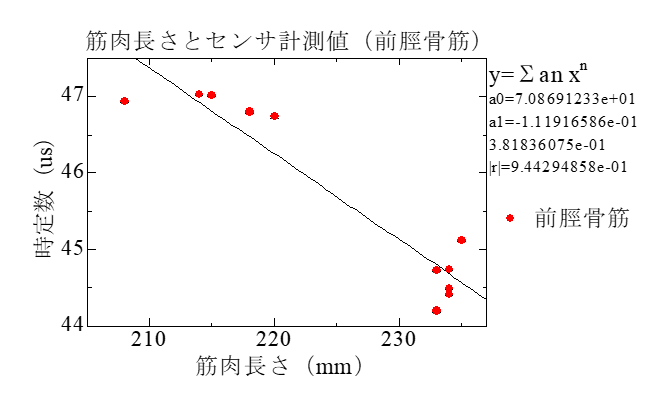
\includegraphics[width=0.78\columnwidth,clip]{./4_consideration/動的試験/zenkei.png}
  \caption{ストレッチセンサ動的計測結果(前脛骨筋)}
  \label{}
\end{figure}

\begin{figure}
  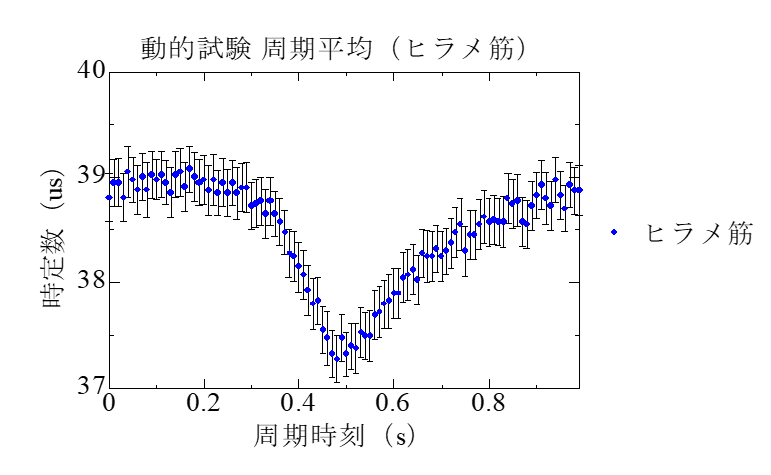
\includegraphics[width=0.78\columnwidth,clip]{./4_consideration/動的試験/hirame.png}
  \caption{ストレッチセンサ動的計測結果(ヒラメ筋)}
  \label{}
\end{figure}


\section{考察}
\subsection{ストレッチセンサ計測精度}
先ほどの結果より,それぞれの計測位置における空気圧人工筋の長さをグラフに表すと,
Fig.\ref{4-ml}の様になった.このグラフから見てわかるように,腓骨筋とヒラメ筋が組となって
前脛骨筋と逆位相のsin波形的動きをさせることが出来た.今回,足関節ロボットの空気圧人工筋
それぞれに対して,Fig.\ref{output_for_test}の出力を出すよう指令を与えたので
システムとして問題なく動いたことがわかる.

\begin{figure}[h]
    \begin{center}
        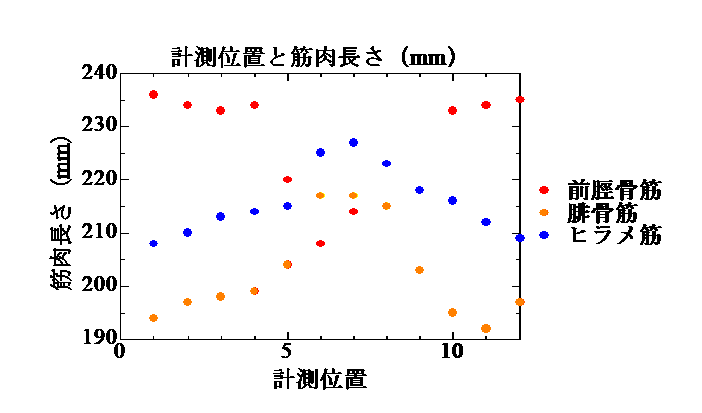
\includegraphics[width=0.78\columnwidth,clip]{4_consideration/ml.eps}
    \end{center}
    \caption{計測位置と各空気圧人工筋の長さの関係}
    \label{4-ml}
\end{figure}

\newpage

続いて,Table.\ref{4_2}の結果を用いて,横軸にセンサの長さ,縦軸に時定数としたグラフを
描画すると,Fig.\ref{ml-rc1},\ref{ml-rc2},\ref{ml-rc3}に示すようになった.
各筋肉に関して,長さが増加するとセンサでの計測値が減少した.
どの筋肉においても同様の結果を示しており,ストレッチセンサが伸びると
静電容量が減少するといったことが分かった.

一方でセンサごとに空気圧人工筋の長さに対する計測値の変化の特性が異なる.これは,
センサ自体が自作されており,その製作時のむらによるものだと考えられる.それに加えて,
空気圧人工筋に設置する時にある程度テンションを与えて設置するのだが,そのテンションの
かけ方具合にもよると考えられる.実際に使用するときは,ストレッチセンサを空気圧人工筋に
設置した状態で,今回の実験の様にセンサ特性の解析を行う必要があると考えられる.

また,空気圧人工筋の伸びの変化に対して,時定数の変化が非常に微小なものとなっている.
今回の時定数の結果や,製作したRC回路の抵抗値$1.5M\Omega$より静電容量の変化量に関して考えると,
最も変化が大きかったヒラメ筋においても$35~38pF$の変化しか現れなかった.
これに対する対策として,RC回路における抵抗値の再選定を行う必要があると考えられた.
抵抗値を増加させると時定数も増加するのでマイコンで変化量を計測しやすくなる.
一方で,抵抗値を増大させると計測ノイズ成分も大きくなるので,その辺りも踏まえて抵抗値の
再選定をしていく必要があると考えられる.

\begin{figure}[h]
    \begin{center}
        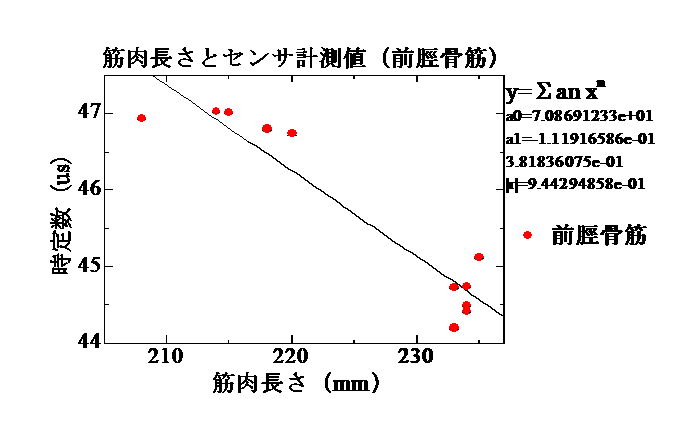
\includegraphics[width=0.78\columnwidth,clip]{4_consideration/zenkei.eps}
    \end{center}
    \caption{空気圧人工筋の長さとセンサ計測値の関係(前脛骨筋)}
    \label{ml-rc1}
\end{figure}

\begin{figure}[h]
    \begin{center}
        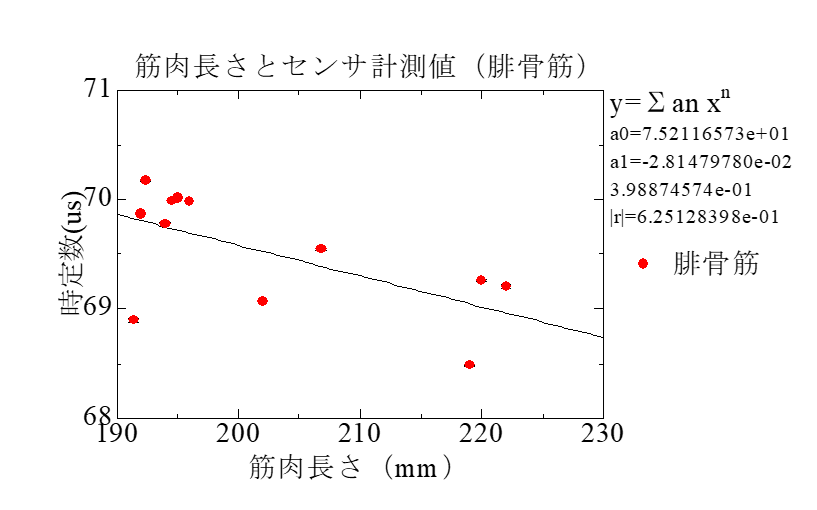
\includegraphics[width=0.78\columnwidth,clip]{4_consideration/hikotsu.eps}
    \end{center}
    \caption{空気圧人工筋の長さとセンサ計測値の関係(腓骨筋)}
    \label{ml-rc2}
\end{figure}

\begin{figure}[h]
    \begin{center}
        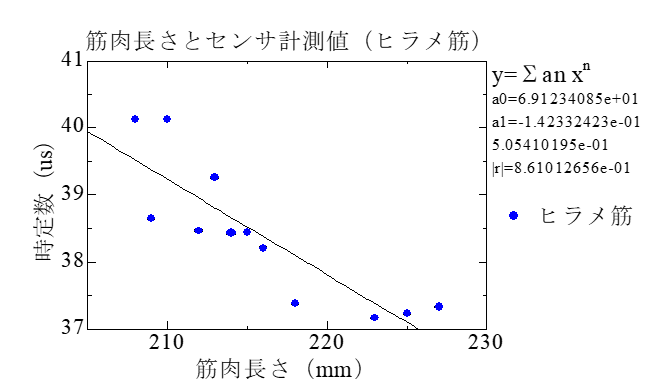
\includegraphics[width=0.78\columnwidth,clip]{4_consideration/hirame.eps}
    \end{center}
    \caption{空気圧人工筋の長さとセンサ計測値の関係(ヒラメ筋)}
    \label{ml-rc3}
\end{figure}

\chapter{結言}
\section{結言}
今回の研究で、足関節ロボットの製作を行い、その底背屈動作の確認を行うことが出来た。
これにより、従来では出来なかった、ヒトの足関節と同様の自由度を持った動きをすることが、
可能になった。

ストレッチセンサ

%#!jlatex main.tex

\chapter*{�ӎ�}
\addcontentsline{toc}{chapter}{�ӎ�}
���������S�ʂɂ킽��C���X�̎����ɕx�ނ�����������C�܂��C��Ɍ����̕������w�������Ē����܂����{�蕶�v�����ɁC�r��Ȃ�ӈӂ�\���܂�.

�����āC�I�m�Ȃ��w���C�������𒸂��܂�������G���u�t�ɐ[�����Ӓv���܂��D

�܂��C���X�̂������𒸂��܂����A���[�T�����Ɋ��ӂ̈ӂ�\���܂��D

�����݂̂Ȃ炸�C���̑��������ʂŐ������̓I�m�Ȃ������𒸂��C��ɖʓ|�����ĉ��������x�i�������ɐ[�����Ӓv���܂��D

�����ɍۂ��A�l�X�Ȃ����͂������������Ґ^�����A�����T�玁�Ɋ��ӂ̈ӂ�\���܂��D

���������S�ʂɂ킽��C���X�̂������𒸂��܂����{�茤�����̊F�l�S���Ɋ��Ӓv���܂��D

�Ō�ɁC���‚��������C�x���Ă��ꂽ���ƕ�Ɋ��ӂ��܂��D


\pagebreak

\begin{thebibliography}{99}
\addcontentsline{toc}{chapter}{\protect \numberline{参考文献}}

%1_introduction

%\bibitem{sample}
%宮研 花子:``○○による××'', 大阪大学修士論文, 20xx
\bibitem{MITSoftRobot} "Textile Silicone Hybrid Sensor Fabrication \newline Guide".soft robotics toolkit. \newline https://softroboticstoolkit.com/resources-for-educators/tsh-sensor ,(参照日 2020-01-02)

\bibitem{kinesiology}
D. A. Nuemann, ``{\it Kinesiology of the Nusculoskeletal System}'', Mosby, 2002.

\bibitem{Crams}
E. Criswell, "{\it Cram's Introduction to Surface Electromyography Second Edition}", Jones \& Bartlett Pub, 2008.

\end{thebibliography}


%\appendix

\chapter{Appendix A}
\section{Section}


%\end{thebibliography}
%\normalsize
%\printindex
\end{document}




